\documentclass[12pt,]{article}
\usepackage{lmodern}
\usepackage{amssymb,amsmath}
\usepackage{ifxetex,ifluatex}
\usepackage{fixltx2e} % provides \textsubscript
\ifnum 0\ifxetex 1\fi\ifluatex 1\fi=0 % if pdftex
  \usepackage[T1]{fontenc}
  \usepackage[utf8]{inputenc}
\else % if luatex or xelatex
  \ifxetex
    \usepackage{mathspec}
  \else
    \usepackage{fontspec}
  \fi
  \defaultfontfeatures{Ligatures=TeX,Scale=MatchLowercase}
    \setmainfont[]{Times New Roman}
\fi
% use upquote if available, for straight quotes in verbatim environments
\IfFileExists{upquote.sty}{\usepackage{upquote}}{}
% use microtype if available
\IfFileExists{microtype.sty}{%
\usepackage{microtype}
\UseMicrotypeSet[protrusion]{basicmath} % disable protrusion for tt fonts
}{}
\usepackage[margin=2.54cm]{geometry}
\usepackage{hyperref}
\hypersetup{unicode=true,
            pdftitle={Examining the Hydrologic Properties of the Missouri River Basin},
            pdfauthor={Rachel Bash, Keqi He, Caroline Watson, and Haoyu Zhang},
            pdfborder={0 0 0},
            breaklinks=true}
\urlstyle{same}  % don't use monospace font for urls
\usepackage{longtable,booktabs}
\usepackage{graphicx,grffile}
\makeatletter
\def\maxwidth{\ifdim\Gin@nat@width>\linewidth\linewidth\else\Gin@nat@width\fi}
\def\maxheight{\ifdim\Gin@nat@height>\textheight\textheight\else\Gin@nat@height\fi}
\makeatother
% Scale images if necessary, so that they will not overflow the page
% margins by default, and it is still possible to overwrite the defaults
% using explicit options in \includegraphics[width, height, ...]{}
\setkeys{Gin}{width=\maxwidth,height=\maxheight,keepaspectratio}
\IfFileExists{parskip.sty}{%
\usepackage{parskip}
}{% else
\setlength{\parindent}{0pt}
\setlength{\parskip}{6pt plus 2pt minus 1pt}
}
\setlength{\emergencystretch}{3em}  % prevent overfull lines
\providecommand{\tightlist}{%
  \setlength{\itemsep}{0pt}\setlength{\parskip}{0pt}}
\setcounter{secnumdepth}{5}
% Redefines (sub)paragraphs to behave more like sections
\ifx\paragraph\undefined\else
\let\oldparagraph\paragraph
\renewcommand{\paragraph}[1]{\oldparagraph{#1}\mbox{}}
\fi
\ifx\subparagraph\undefined\else
\let\oldsubparagraph\subparagraph
\renewcommand{\subparagraph}[1]{\oldsubparagraph{#1}\mbox{}}
\fi

%%% Use protect on footnotes to avoid problems with footnotes in titles
\let\rmarkdownfootnote\footnote%
\def\footnote{\protect\rmarkdownfootnote}

%%% Change title format to be more compact
\usepackage{titling}

% Create subtitle command for use in maketitle
\providecommand{\subtitle}[1]{
  \posttitle{
    \begin{center}\large#1\end{center}
    }
}

\setlength{\droptitle}{-2em}

  \title{Examining the Hydrologic Properties of the Missouri River Basin}
    \pretitle{\vspace{\droptitle}\centering\huge}
  \posttitle{\par}
  \subtitle{\url{https://github.com/cwatson1013/Hydrologic_Data_Analysis_Final_Proj}}
  \author{Rachel Bash, Keqi He, Caroline Watson, and Haoyu Zhang}
    \preauthor{\centering\large\emph}
  \postauthor{\par}
    \date{}
    \predate{}\postdate{}
  
\usepackage{booktabs}
\usepackage{longtable}
\usepackage{array}
\usepackage{multirow}
\usepackage{wrapfig}
\usepackage{float}
\usepackage{colortbl}
\usepackage{pdflscape}
\usepackage{tabu}
\usepackage{threeparttable}
\usepackage{threeparttablex}
\usepackage[normalem]{ulem}
\usepackage{makecell}
\usepackage{xcolor}

\usepackage{float}

\begin{document}
\maketitle

\newpage

\hypertarget{rationale-and-research-questions}{%
\section{Rationale and Research
Questions}\label{rationale-and-research-questions}}

The Missouri River is the largest river in North America (2,540 miles)
and has the second largest watershed spanning 529,000
<<<<<<< HEAD
mi\textsuperscript{2} ((Kammerer 1990)). Its watershed covers portions
of ten states, which account for approximately one-sixth of the
continental United States, as well as a small part of Canada (U.S. Army
Corps of Engineers Missouri River Basin Water Management Division 2018).
The headwater is located in the Bitterroot Mountains River of
northwestern Wyoming and southwestern Montana (Committee on Missouri
River Ecosystem Science 2002). The basin is primarily rural, but also
has several large and medium-sized cities. In 2012, the basin was home
to approximately 15.5 million people, and many large cities in the
region are in proximity to the Missouri River (U.S. Army Corps of
Engineers Missouri River Basin Water Management Division 2018). Demands
for managing the river for the benefit of human livelihood has resulted
in drastic modification in the river and the floodplains. Now, the river
is used intensively in multiple ways, including municipal, agricultural,
hydropower, recreation, flood control etc. (Bureau of Reclamation
2016b).
=======
mi\textsuperscript{2} ({[}@kammerer1990{]}). Its watershed covers
portions of ten states, which account for approximately one-sixth of the
continental United States, as well as a small part of Canada
{[}@usace2018{]}. The headwater is located in the Bitterroot Mountains
River of northwestern Wyoming and southwestern Montana {[}@nrc2002{]}.
The basin is primarily rural, but also has several large and
medium-sized cities. In 2012, the basin was home to approximately 15.5
million people, and many large cities in the region are in proximity to
the Missouri River {[}@usace2018{]}. Demands for managing the river for
the benefit of human livelihood has resulted in drastic modification in
the river and the floodplains. Now, the river is used intensively in
multiple ways, including municipal, agricultural, hydropower,
recreation, flood control etc. {[}@bor2016-1{]}.
>>>>>>> 5d321b88819c6cf0c8ae22b21efafc6a4c9de8b3

Within the 328 million acres of the basin's total area in the United
States, 64.2\% are related to agricultural uses, while the rest are
dedicated for recreation, fish and wildlife, and urban development
<<<<<<< HEAD
(Bureau of Reclamation 2016b). 37.1\% of the total basin area is pasture
and range grassland primarily for grazing, and cropland consists of
almost 92 million acres (U.S. Army Corps of Engineers Missouri River
Basin Water Management Division 2018). As of 2012, irrigated land
comprises 14.2 million acres, and require a delivery of about 13 million
acre-feet of surface water annually (U.S. Army Corps of Engineers
Missouri River Basin Water Management Division 2018). Wetlands and water
bodies, on the other hand, cover 3.7 and 1.8 million acres, respectively
(U.S. Army Corps of Engineers Missouri River Basin Water Management
Division 2018). In spite of the low proportion of water areas (2.3\%),
=======
{[}@bor2016-1{]}. 37.1\% of the total basin area is pasture and range
grassland primarily for grazing, and cropland consists of almost 92
million acres {[}@usace2018{]}. As of 2012, irrigated land comprises
14.2 million acres, and require a delivery of about 13 million acre-feet
of surface water annually {[}@usace2018{]}. Wetlands and water bodies,
on the other hand, cover 3.7 and 1.8 million acres, respectively
{[}@usace2018{]}. In spite of the low proportion of water areas (2.3\%),
>>>>>>> 5d321b88819c6cf0c8ae22b21efafc6a4c9de8b3
they are the pivotal foundation for agricultural or other usages, and
thus critical to the whole region's economy.

The agricultural, urban, and industrial development in the region
inevitably causes nutrient loading and enrichment in water bodies,
especially for nitrogen (N) and phosphorus (P). Agricultural input
through fertilizer is the predominant anthropogenic source for nutrient
<<<<<<< HEAD
in water bodies in the whole basin (Committee on Missouri River
Ecosystem Science 2002). Regardless of the major anthropogenic source,
nutrient enrichment is considered nationally as one of the leading
factors for water quality impairment. According to the Clean Water Act
303(d) lists (2015), more than 160 stream reaches or waterbodies were
reported by USEPA to suffer nutrient-related impairment in 2015.
=======
in water bodies in the whole basin {[}@nrc2002{]}. Regardless of the
major anthropogenic source, nutrient enrichment is considered nationally
as one of the leading factors for water quality impairment. According to
the Clean Water Act 303(d) lists (2015), more than 160 stream reaches or
waterbodies were reported by USEPA to suffer nutrient-related impairment
in 2015.
>>>>>>> 5d321b88819c6cf0c8ae22b21efafc6a4c9de8b3

In addition to change in nutrient concentration, discharge appears to be
highly variable in the basin, and both severe drought and flooding
events have occurred in the basin regularly. For example, in the spring
and summer of 2011, an unprecedented flooding event caused over \$2
billion damage and 5 fatalities, leading to FEMA disaster declaration
<<<<<<< HEAD
made in all states along the Missouri River (National Oceanic and
Atmospheric Administration 2012). During the flooding event, around
11,000 people evacuated from Minot, North Dakota owing to high water
level in Souris River, which flooded 4,000 homes (National Oceanic and
Atmospheric Administration 2012). In 2012, a drought struck the Central
Great Plain, including the basin, and inflicted at least \$12 billion of
agricultural loss before July, 2012 (NOAA Drought Task Force 2013).
Recently, another flooding event occurred in the spring of 2018, due to
the months of January through May being the wettest period on record for
the U.S.
=======
made in all states along the Missouri River {[}@noaa2012{]}. During the
flooding event, around 11,000 people evacuated from Minot, North Dakota
owing to high water level in Souris River, which flooded 4,000 homes
{[}@noaa2012{]}. In 2012, a drought struck the Central Great Plain,
including the basin, and inflicted at least \$12 billion of agricultural
loss before July, 2012 {[}@noaa2013{]}. Recently, another flooding event
occurred in the spring of 2018, due to the months of January through May
being the wettest period on record for the U.S.
>>>>>>> 5d321b88819c6cf0c8ae22b21efafc6a4c9de8b3

Given all the background information above, we would like to know the
current state of Missouri River and its tributaries, with a focus on the
changing patterns in discharge and nutrient levels. Water bodies along
the downstream are more likely to be impaired by nutrients accumulated
from the upstream. Croplands and pastures, which can further load
nutrients into streams, are distributed throughout the lower basin
(\autoref{fig:cropland}). Therefore, in the present project, study sites
were concentrated in the southeast of the whole Missouri Basin. By
analyzing data retrieved from these sites, we first revealed the general
yearly discharge pattern and changes in variability over years. Then we
investigated how the dramatic change in discharge (i.e.~water quantity)
could potentially interact with nutrient enrichment (i.e.~water
quality). We examined a few specific flooding and drought events, during
which changes in both water quality and quantity were well recorded, so
that we could make inference on the interplay between quantity and
quality. The effect of population on nutrient enrichment was also
examined to illustrate potential non-agricultural impact from human
activities. Finally, based on the pattern in the past and the best model
we could fit, we attempted to predict the likely future conditions and
trends in the Missouri River Basin. Our research questions and
acccompanying hypotheses are below:

\begin{enumerate}
\def\labelenumi{\arabic{enumi}.}
\item
  How have changes in discharge (i.e.~water quantity) interacted with
  nutrient enrichment (i.e.~water quality) in the Missouri River Basin?

  \begin{enumerate}
  \def\labelenumii{\alph{enumii})}
  \tightlist
  \item
    Nutrient levels have increased over time
  \item
    Discharge has become more variable over time
  \item
    Nutrient levels increase with discharge
  \end{enumerate}
\item
  What effects do specific flood and drought events have on the water
  quality and quantity of rivers in the Missouri River Basin areas of
  interest?

  \begin{enumerate}
  \def\labelenumii{\alph{enumii})}
  \tightlist
  \item
    Rivers will exhibit a flushing behavior due to the land use and type
    of flow during storms
  \item
    Discharge will decrease during drought due to decreased overland
    flow.
  \end{enumerate}
\item
  What factors contribute to the variability of total nitrogen in the
  rivers?

  \begin{enumerate}
  \def\labelenumii{\alph{enumii})}
  \tightlist
  \item
    Land use, year, discharge, phosphorus, and HUC region will
    contribute to the variability of total nitrogen across sites
  \end{enumerate}
\item
  Given past and current data, what can we predict about the future
  state of water in the Missouri River Basin?

  \begin{enumerate}
  \def\labelenumii{\alph{enumii})}
  \tightlist
  \item
    Total flow in the Missouri River Basin is increasing
    (non-stationary) over time
  \item
    The future situation of the river basin will see the continuation of
    current trends of increasing overall volume of flow.
  \end{enumerate}
\end{enumerate}

\begin{figure}[H]
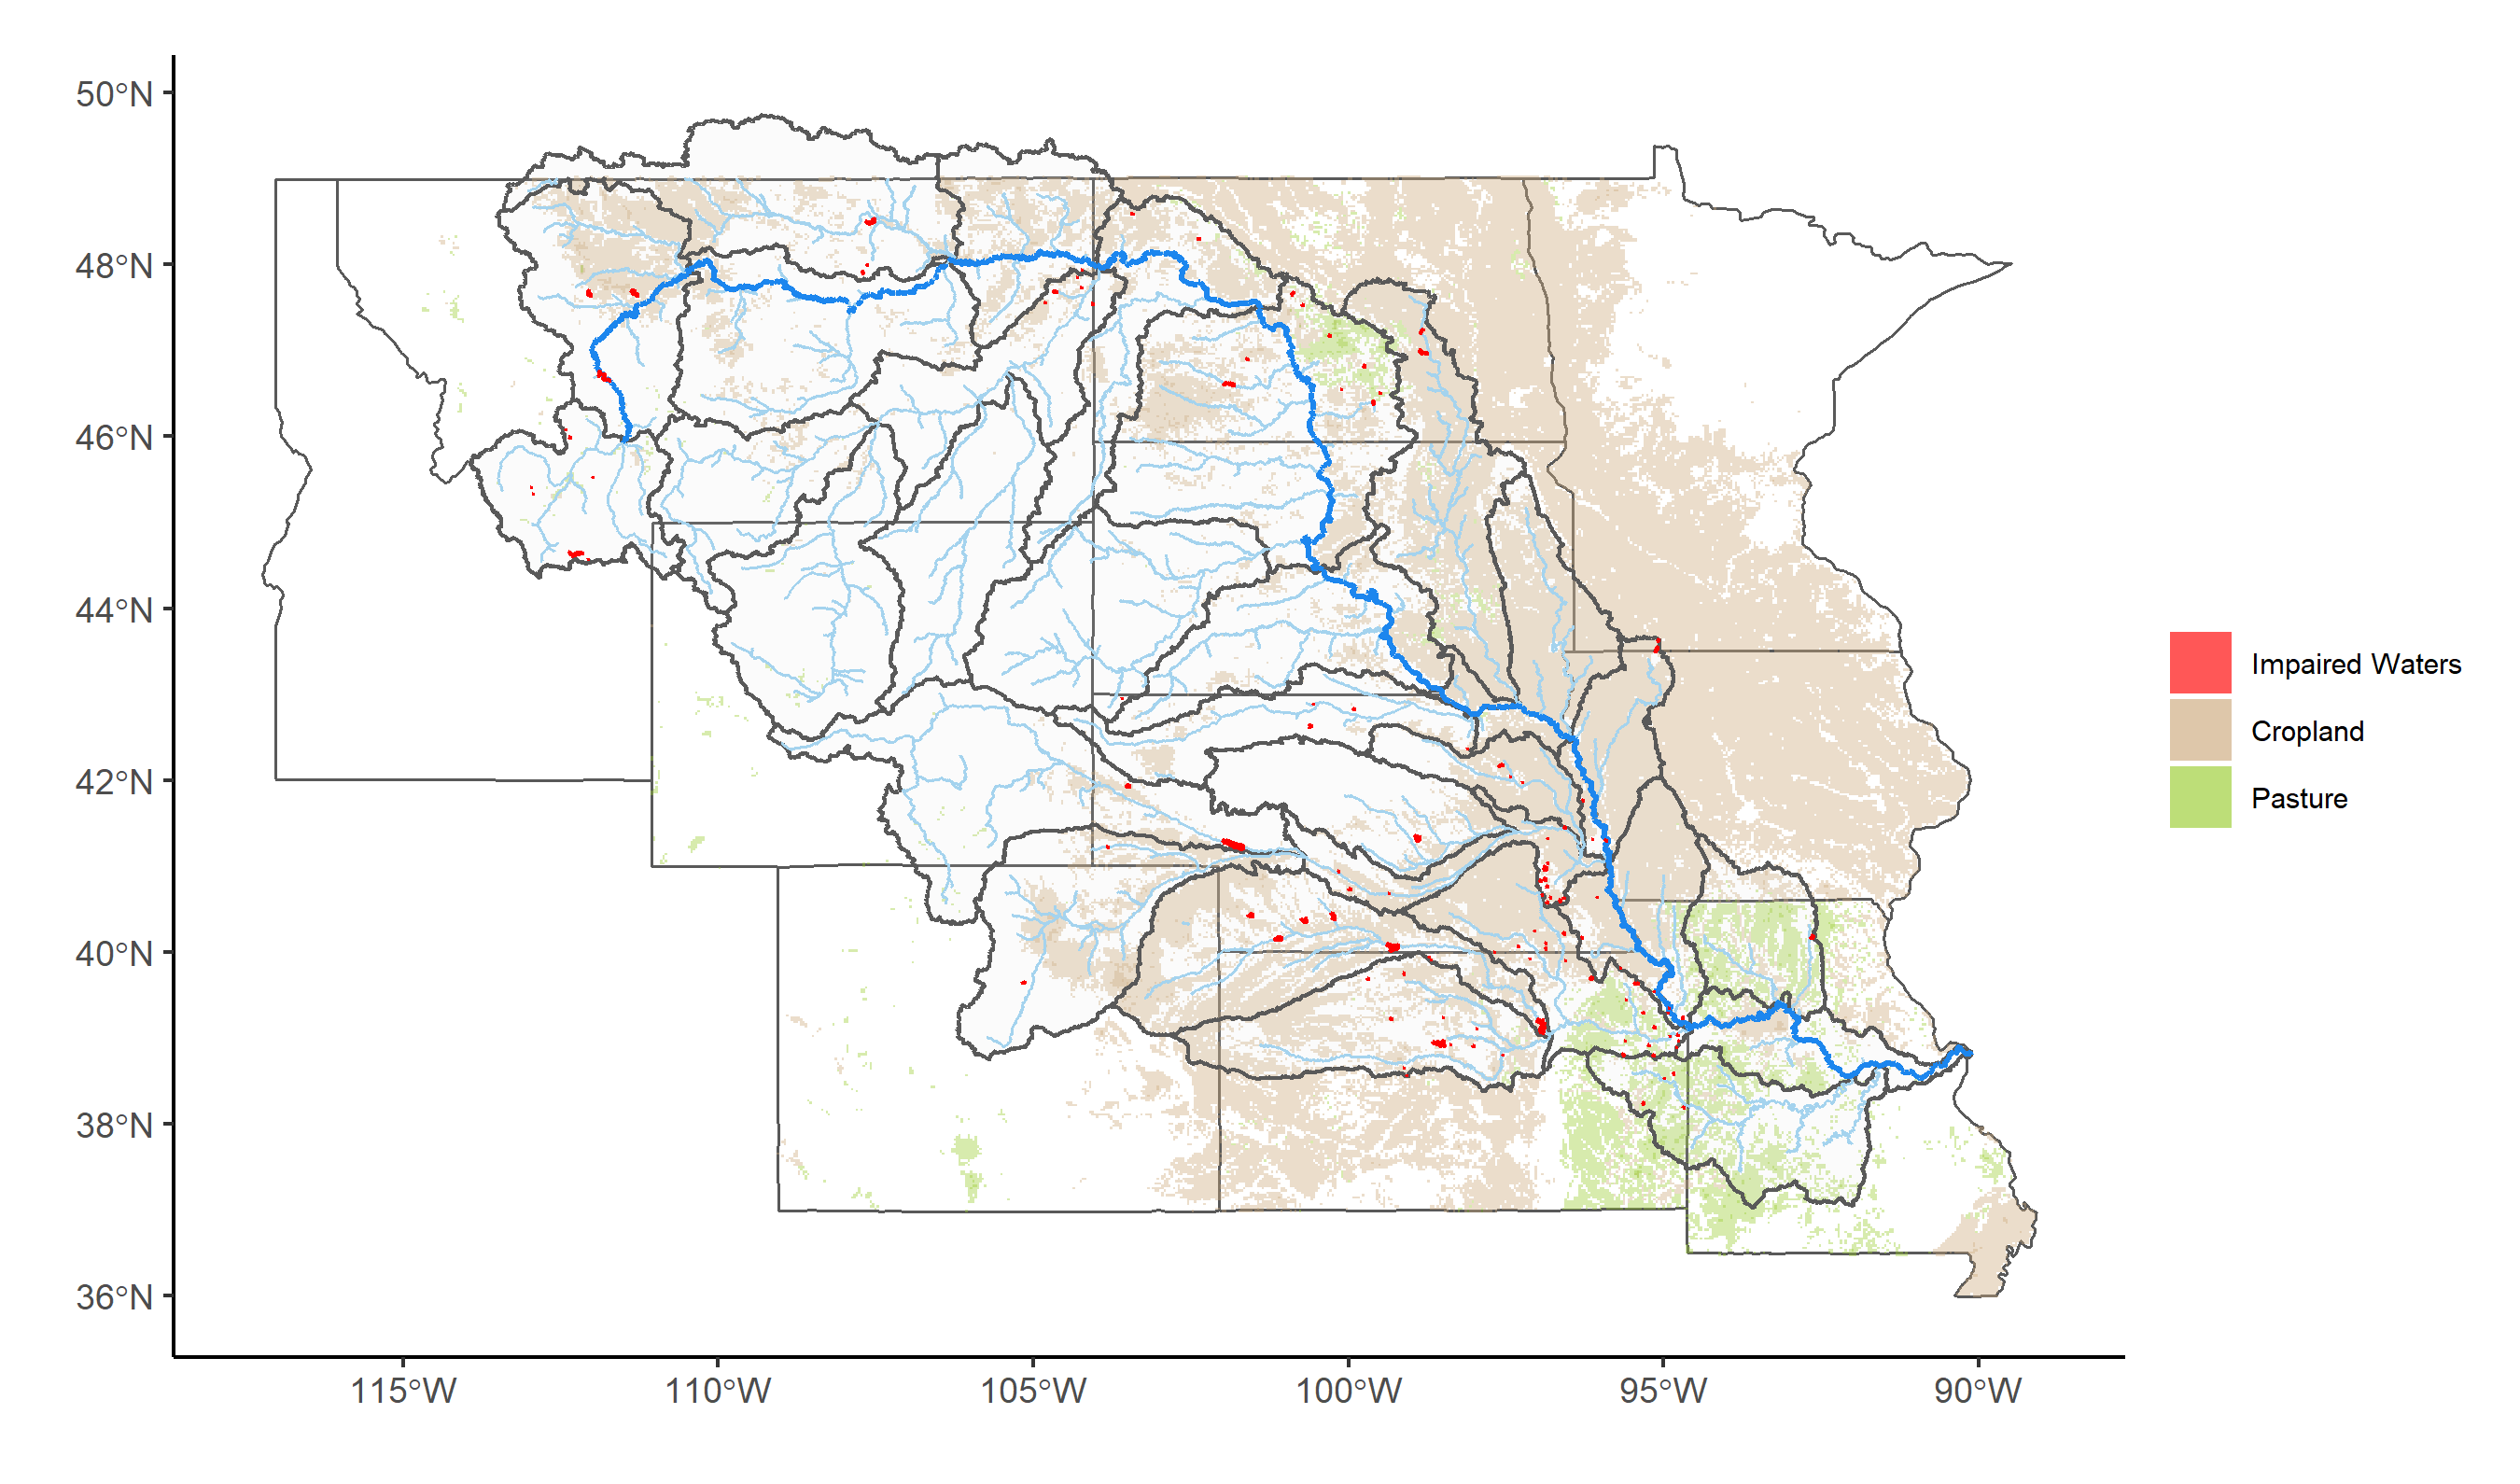
\includegraphics[width=\maxwidth]{../Figures/cropland3} \caption{\label{fig:cropland} Map of agricultural lands and impaired waters in the Missouri River Basin. Row and Close Grain Crop Cultural Formation shown by tan-colored areas, pasture and hay field shown by yellowgreen areas, imparied water bodies according to Clean Water Act Section 303(d) (EPA 2015) denoted by red areas, and all HUC4 watersheds in the Missouri River Basin (1001-1030) delineated by gray polygons. The thin, light-blue lines outline all streams of a Strahler order higher than 2, and the thick blue line represents the mainstem of Missouri River.}\label{fig:cropland}
\end{figure}

\newpage

\hypertarget{dataset-information}{%
\section{Dataset Information}\label{dataset-information}}

The data we are analyzing comes from the United States Geological Survey
(USGS) database called the National Water Information System interface,
or NWIS. We pulled data from the interface using the R package
\texttt{dataRetrieval}. Because we are interested in the southern part
of the Missouri River basin, we pulled sites from each HUC4 subbasin
from 1020 to 1030. We chose these subbasins because they had a variety
of tributaries that all flowed into the Missouri River, representing a
variety of river sizes and lengths. We filtered these subbasin queries
to only show us sites that contained discharge, nitrogen, and phosphorus
data. Once we found the sites with all of this data, we chose 2 sites
from each HUC sub basin for a total of 22. We chose the two sites from
each HUC sub basin by comparing the periods of records for each of our
chosen variables and finding the sites with the longest periods of
records. We chose to look at two sites per HUC region (for a total of
22) in order to maintain a digestible scope (\autoref{fig:sitemap}). We
retrieved data on water quantity and water quality (N, P concentrations)
(Table 1).

Only six sites within our HUC subbasin boundary contained any high
frequency nitrogen data. Therefore, we also looked at these six sites in
order to do analyses and answer our research question about flooding.
Since flooding and droughts can be thought of as opposites, we looked at
the same 6 sites for droughts as we did for flooding (Table x - add
table??).

We have two main datasets:

\begin{itemize}
\item
  The daily values dataset containing discharge, nitrogen, and
  phosphorus data for 22 sites.
\item
  The high freqency dataset containing high frequency data for nitrogen
  and discharge for 6 sites.
\end{itemize}

\textbf{Table 1:} Add title Variable \textbar{} Unit \textbar{} Number
of Sites \textbar{}\\
----------- \textbar{} :---------------: \textbar{} ---------------
\textbar{} Discharge \textbar{} cfs or \(m^{3}\)/s \textbar{} 22 Time
\textbar{} UTC \textbar{} 22 Nitrogen \textbar{} mg/L \textbar{} 22 with
daily values, 6 with high frequency values Phosphorus \textbar{} mg/L
\textbar{} 22

\textbf{Table 2:} Add table for date ranges and possibly sites used for
flooding?

\begin{figure}[H]
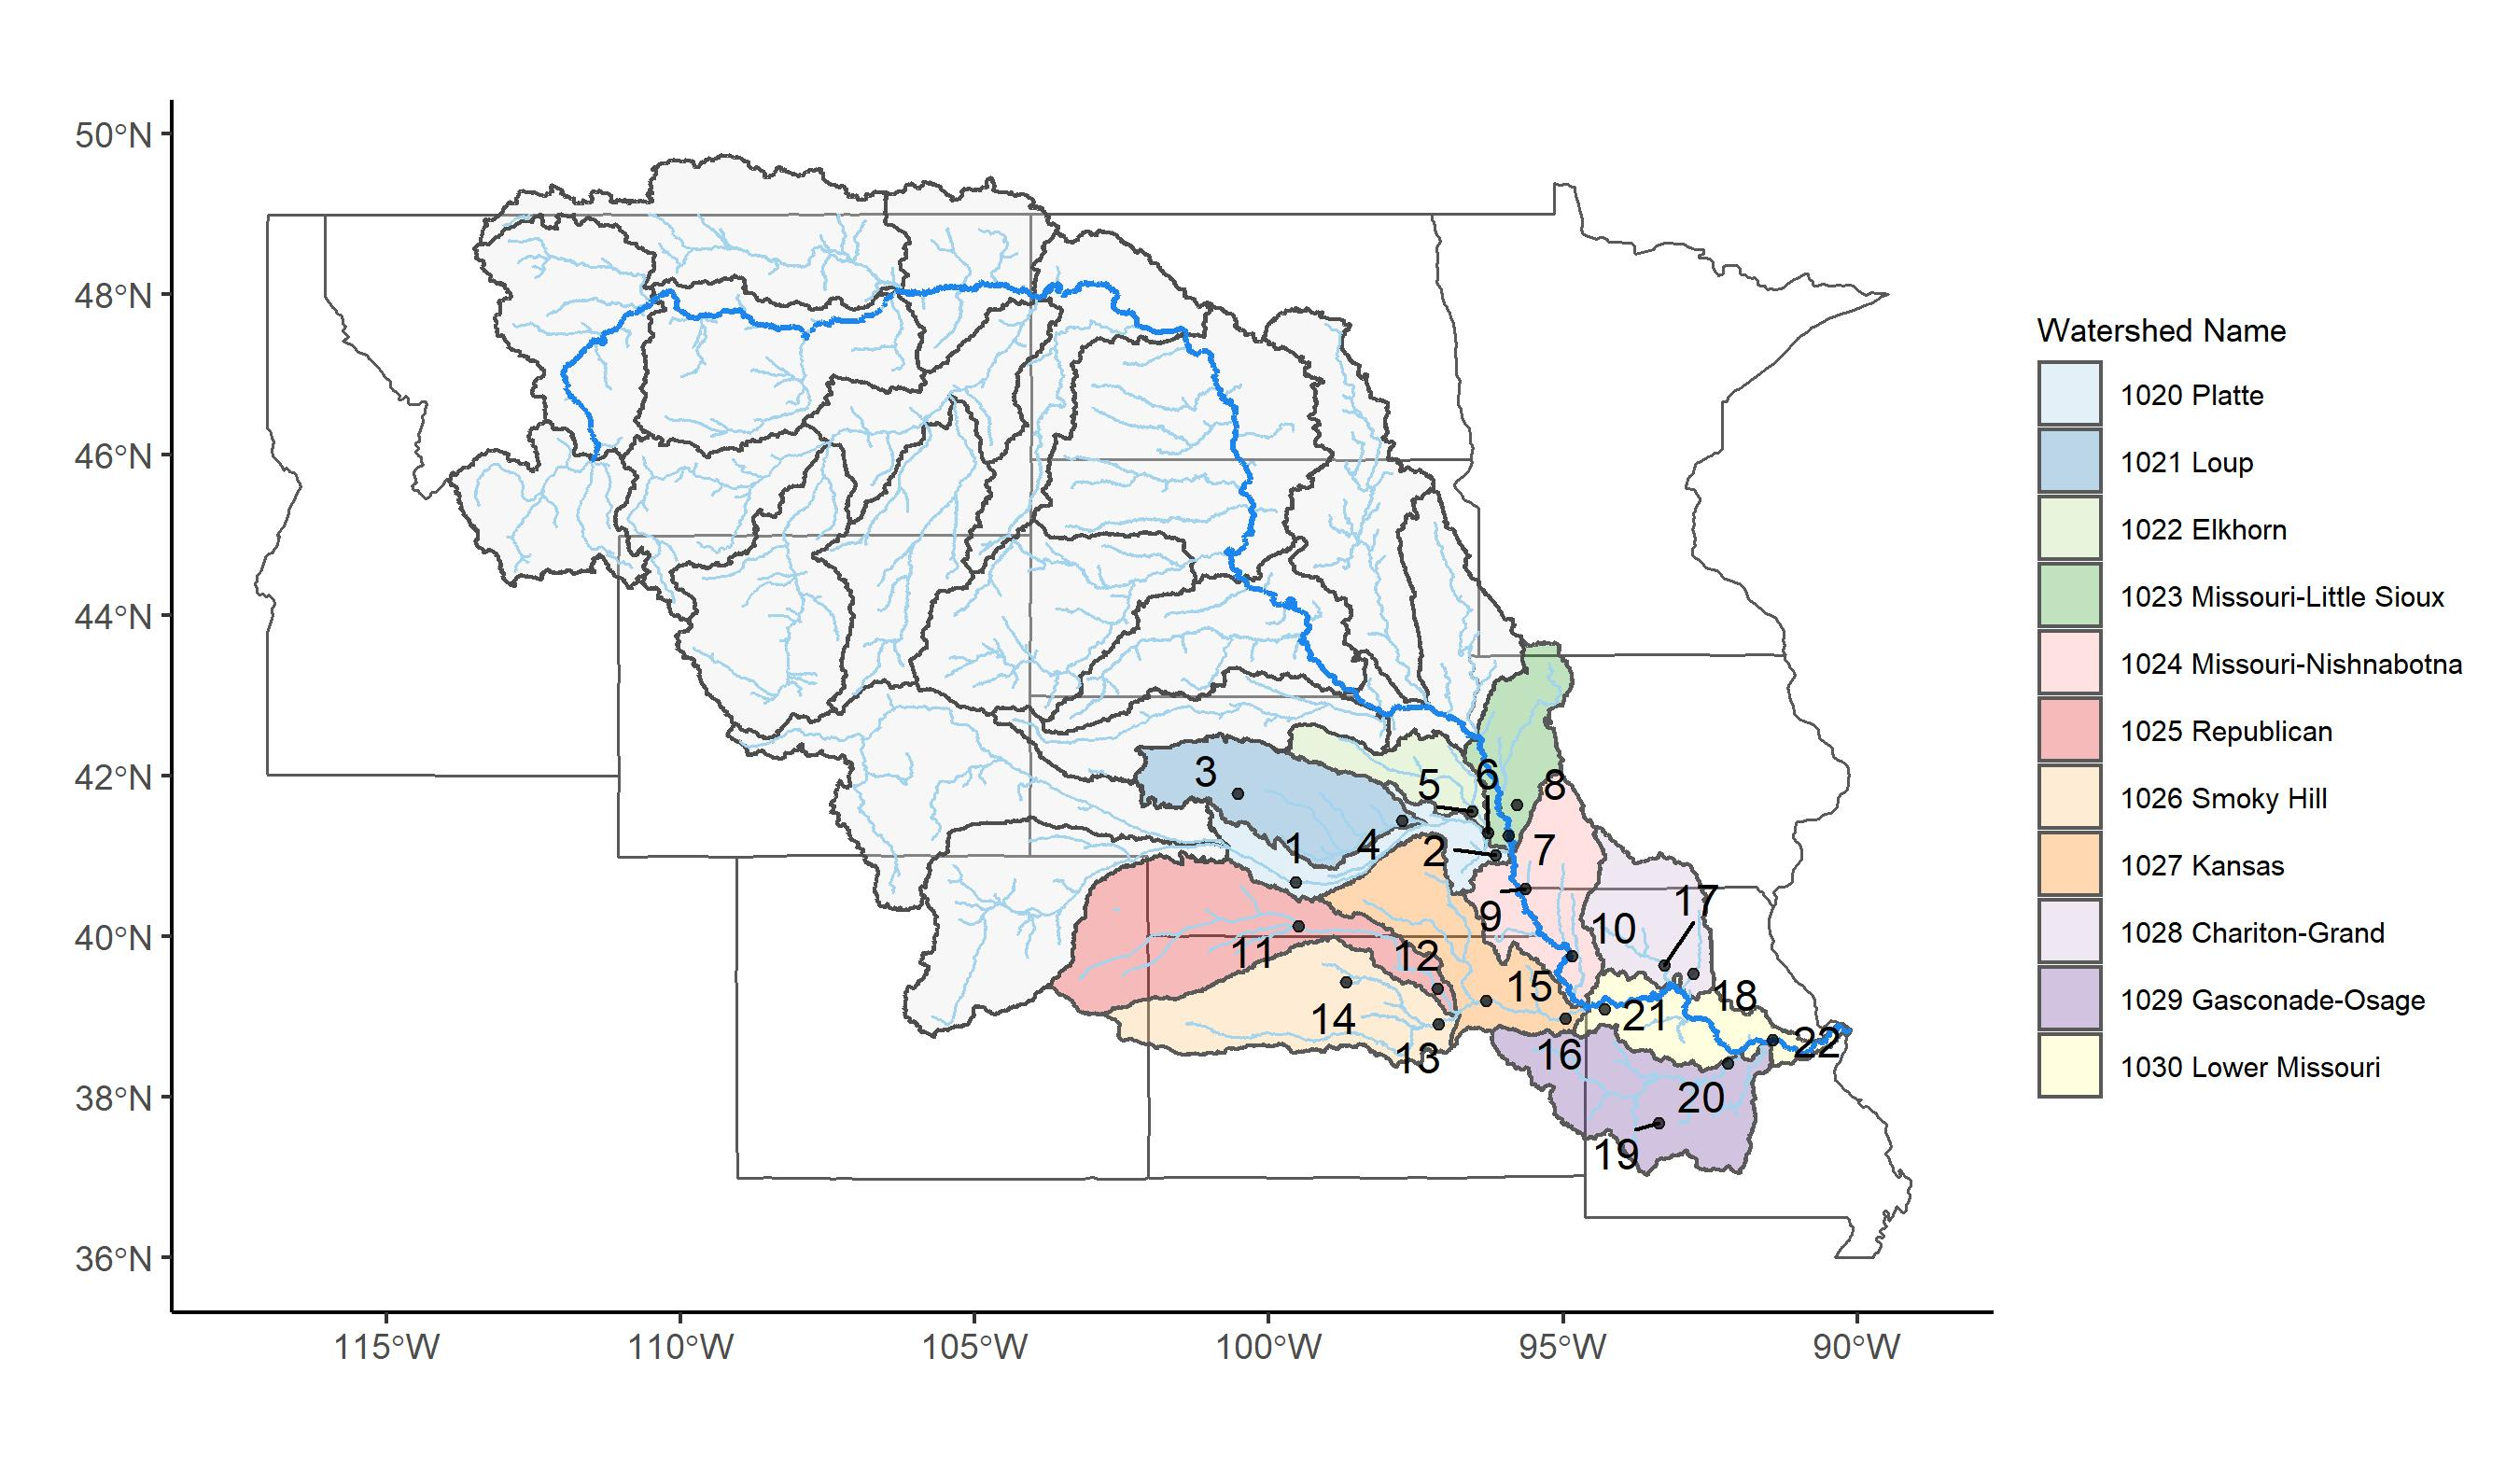
\includegraphics[width=\maxwidth]{../Figures/site_map} \caption{\label{fig:sitemap} Map of USGS sites used for long term analysis.}\label{fig:sitemap}
\end{figure}

\newpage

\hypertarget{exploratory-analysis}{%
\section{Exploratory Analysis}\label{exploratory-analysis}}

\hypertarget{exploration-of-variables}{%
\subsection{Exploration of variables}\label{exploration-of-variables}}

Basic data wrangling was needed in order to obtain all variables of
interest. After obtaining all pertinent data, each variable was
visualized in order to see the shape of the data and the range of values
(\autoref{fig:Nhist}). Any necessary transformation or cleaning was
completed after this step.

\begin{figure}[H]
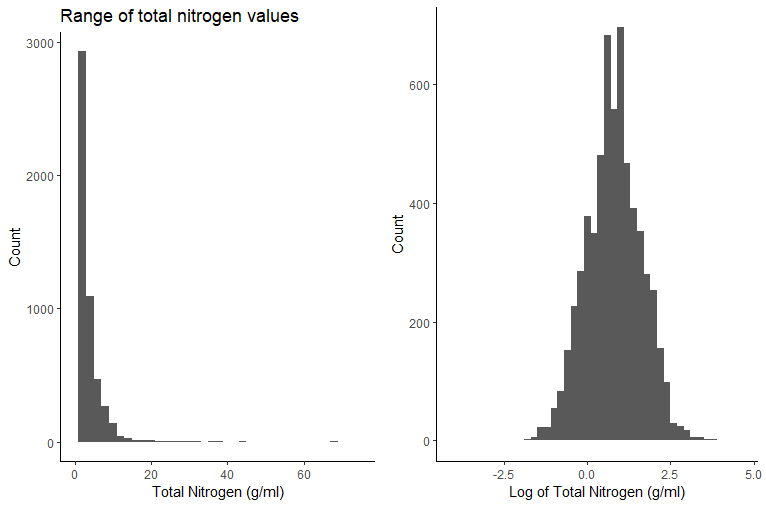
\includegraphics[width=\maxwidth]{../Figures/Nitrogenhist} \caption{\label{fig:Nhist} Histograms showing the range of total nitrogen values obtained from all sites during the total period of record. Raw (left) and logged (right) nitrogen data are shown to show that any analysis requiring normally distributed data will use the log transformed nitrogen data.}\label{fig:Nhist}
\end{figure}

Discharge, nitrogen, and phosphorus were plotted for each site and
examined together in order to see if there were any obvious patterns or
trends (\autoref{fig:dataexample}).

\begin{figure}[H]
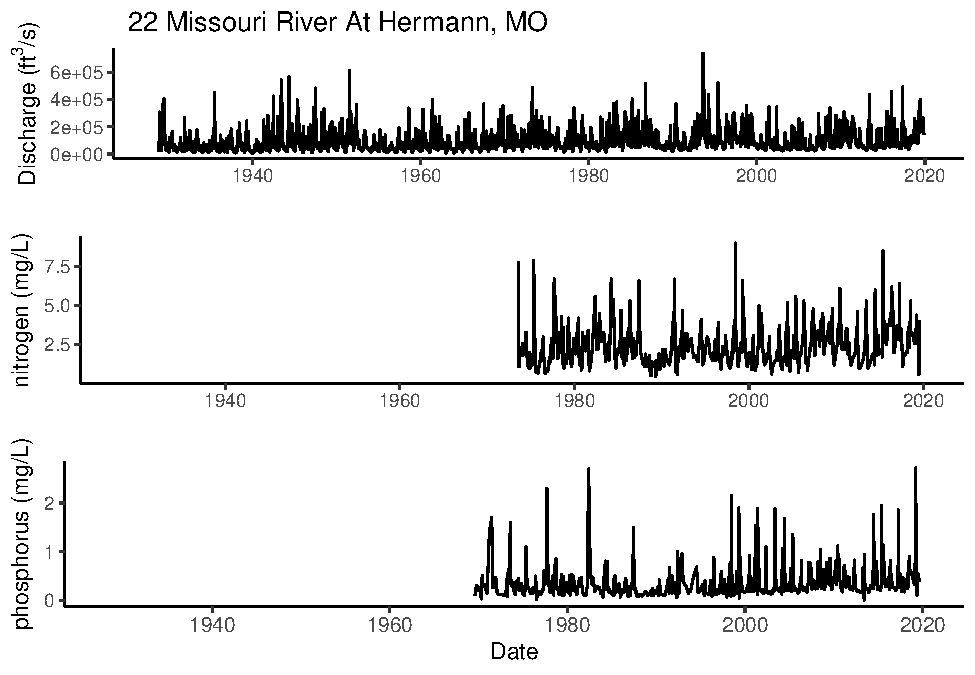
\includegraphics[width=\maxwidth]{Missouri-Reasearch-Project---FINAL_files/figure-latex/dataexample-1} \caption{\label{fig:dataexample} Discharge, Nitrogen, Phosphorus daily data of Site No. 22, the  Missouri River At Hermann, MO.}\label{fig:dataexample}
\end{figure}

\hypertarget{yearly-discharge-pattern}{%
\subsection{Yearly Discharge Pattern}\label{yearly-discharge-pattern}}

Typical discharge patterns within a year for each HUC4 watershed from
1020 to 1030 were generated by compiling all available discharge data at
the 22 selected USGS site (\autoref{fig:dispattern}). Generally,
discharge reaches its peak during the summer and falls to minima during
the winter, and most of the sites exhibit rather high variations across
years, as indicated by the large difference between the medians and the
first or the third quartiles. Furthermore, highest variations in
discharge appear to occur in the summer, whereas discharge in the winter
varies less among years. The large variability within a year and the
seasonal pattern is only obvious in larger streams and rivers but not in
small creeks (e.g.~site 5 Maple Creek near Nickerson, site 8 Boyer
River, site 21 Small Blue River). Exceptions to the generalization are
three sites with medium discharge (site 1 Platte River, NE; site 3
Dismal River, NE; site 11 Republican River, NE). They have fairly
constant discharge and variation across years, and the the first and the
third even have slightly lower discharge during the summer. Platte River
forms by the confluence of North Platte and South Platte Rivers, and
both two have snowmelt as their water source, resulting in the observed
higher discharge during the spring and low in the summer. Dismal River
forms by two forks that arise from groundwater (Ogallala Aquifer), which
is supposed to be more stable than precipitation. The majority of
<<<<<<< HEAD
Republican River basin is underlain by Ogallala Aquifer (Bureau of
Reclamation 2016a), and a plausible high proportion of water source from
=======
Republican River basin is underlain by Ogallala Aquifer
{[}@bor2016-2{]}, and a plausible high proportion of water source from
>>>>>>> 5d321b88819c6cf0c8ae22b21efafc6a4c9de8b3
groundwater could explain the little variation across years.

\begin{figure}[H]
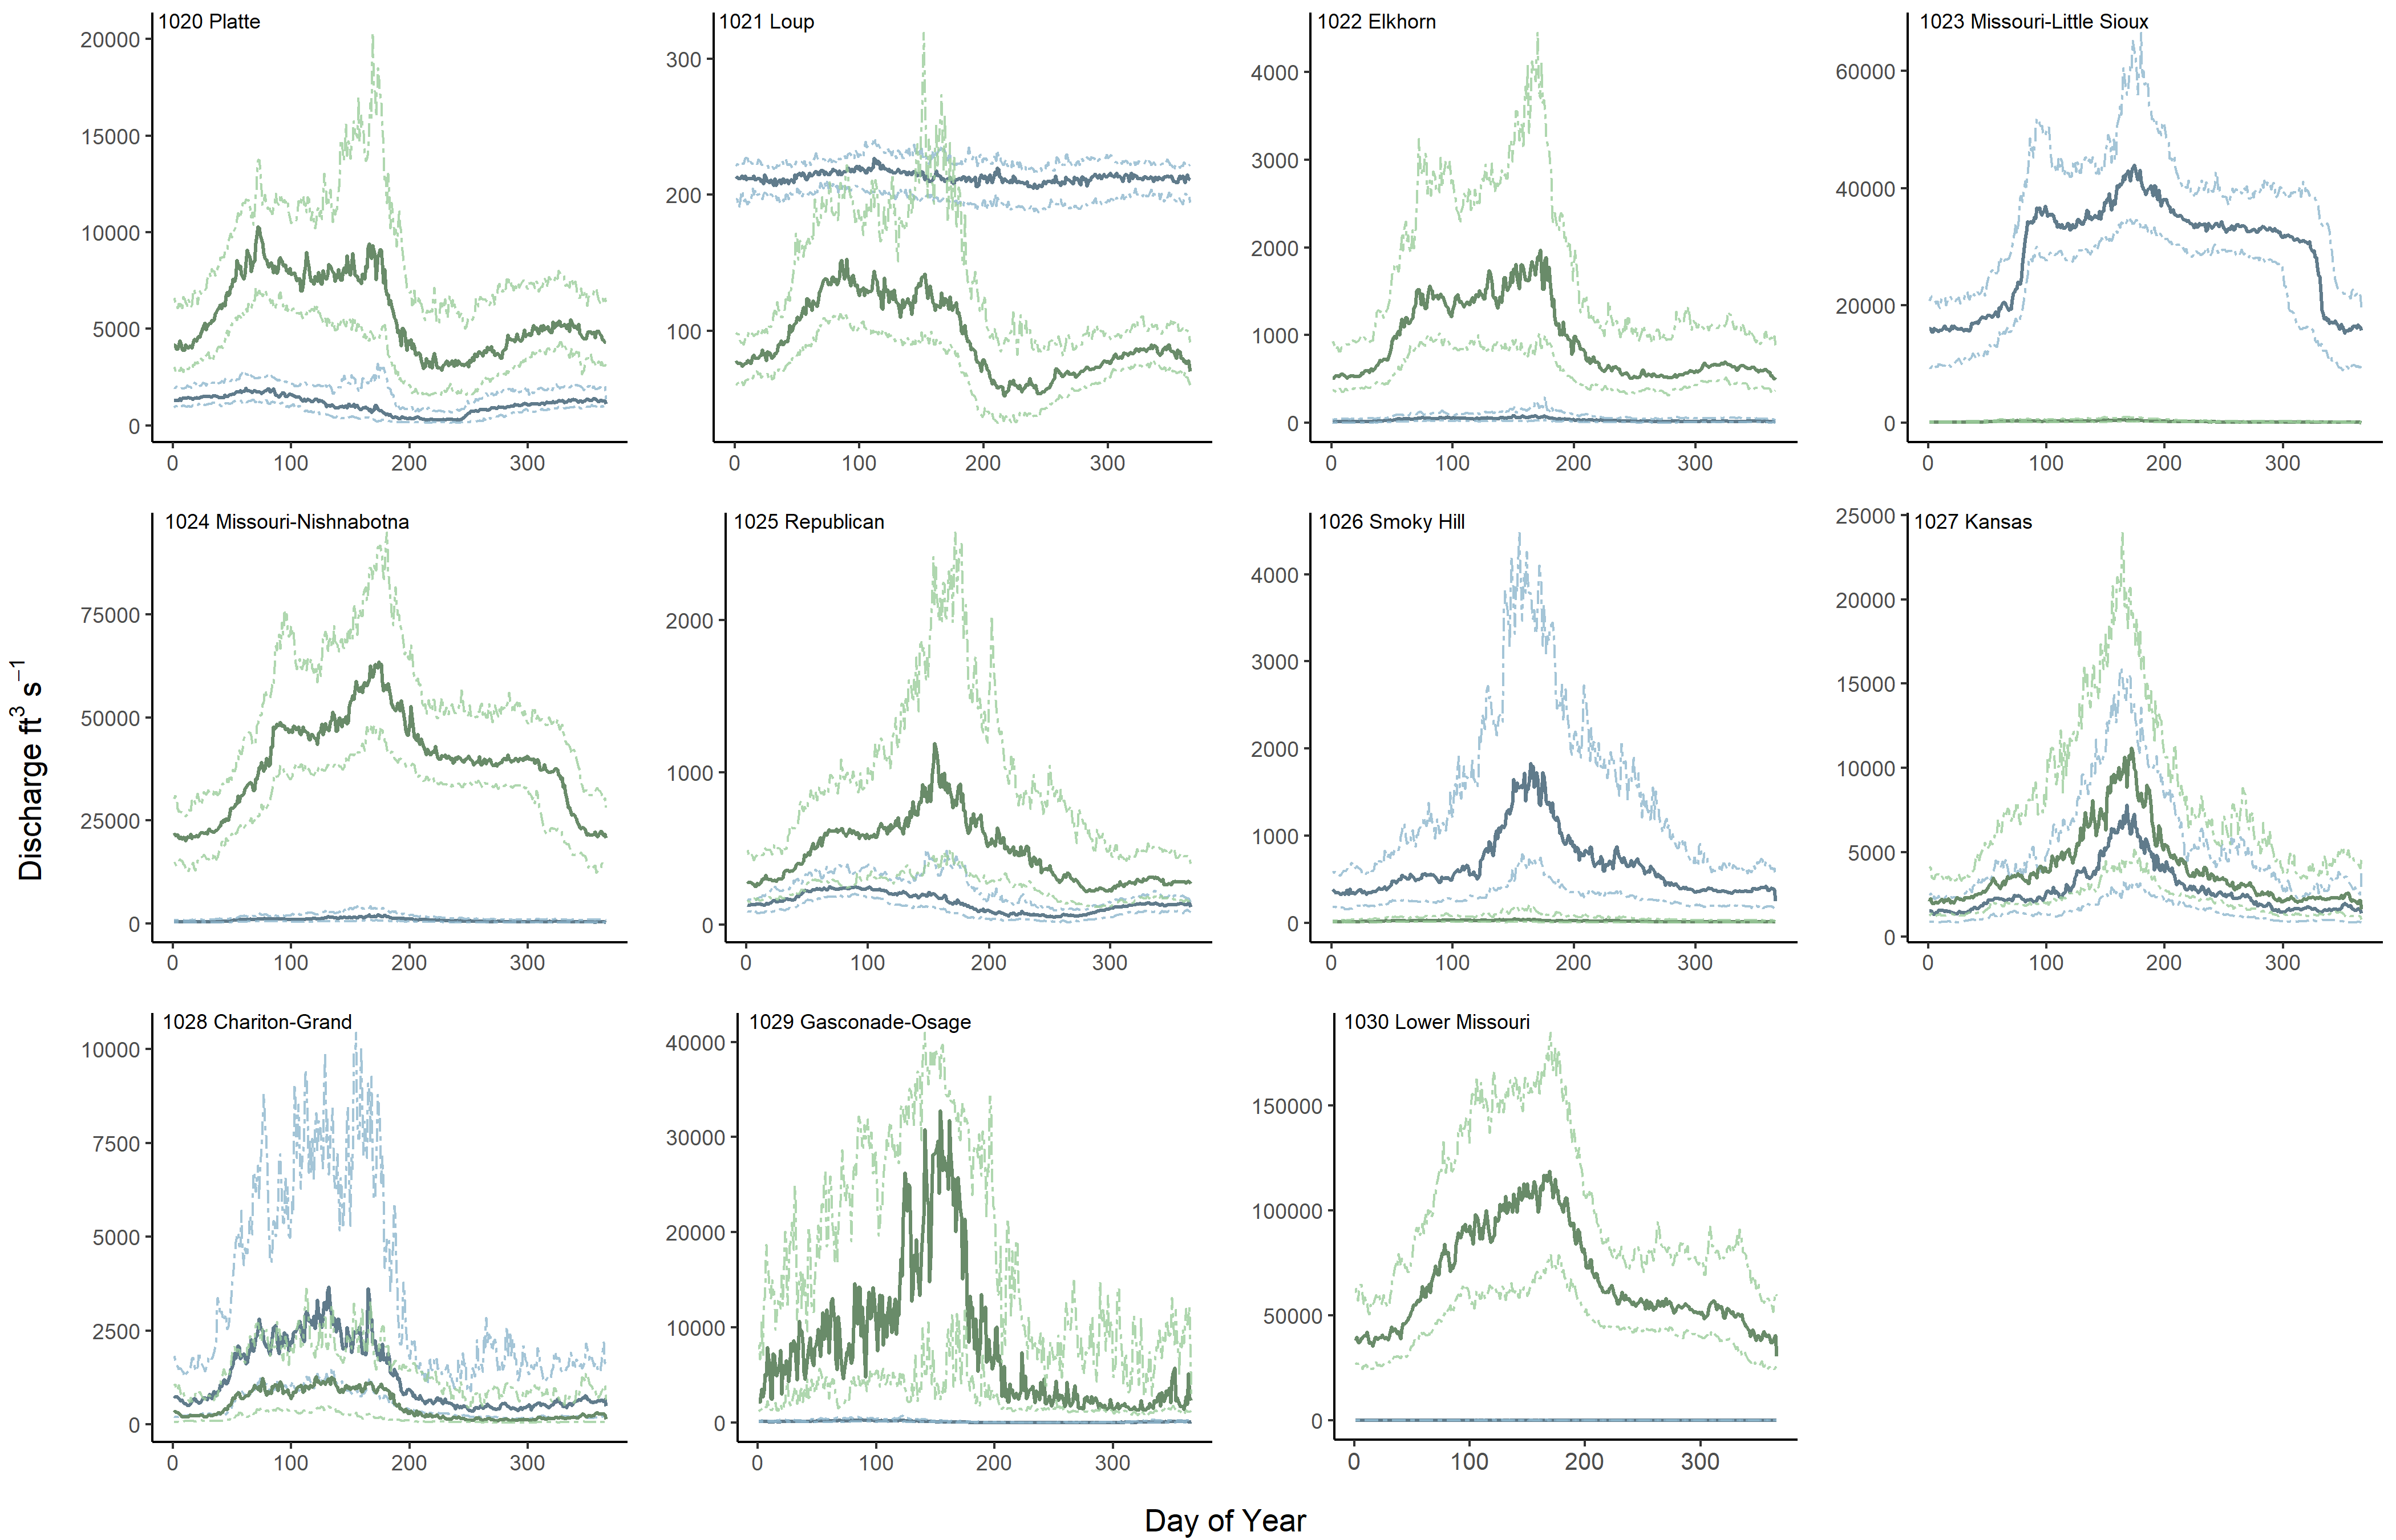
\includegraphics[width=\maxwidth]{../Figures/discharge} \caption{\label{fig:dispattern}Yearly discharge pattern for the lower Missouri HUC4 watersheds. Thick, solid, and dark lines are the median of all discharge records on a day of year, while thin, dashed, and light lines are the 25th and 75th discharge quantiles on that day. The blue lines represent the first site in a HUC4 watershed, while the green lines represent the second site.}\label{fig:dispattern}
\end{figure}

\hypertarget{change-in-discharge-variations-over-years}{%
\subsection{Change in Discharge Variations over
Years}\label{change-in-discharge-variations-over-years}}

To reveal how variability of discharge has changed over time, we
analyzed the relationship between standard deviation (SD) of discharge
within a year and years, using linear models (\autoref{fig:varfig};
\autoref{tab:vartab}). Among all the 22 sites, 14 sites suggest
increasing SD over time, and 4 of them show statistically significant
increase. By contrast, only 8 sites suggest declining SD trends, and 2
of them exhibit statistically significant rising in SD. Despite that
only data from six sites (around 27\%) yield conclusive results, within
these sites the number of streams that have become more variable are two
times as many as those with decreasing variability. Thus, our results
suggest that the whole Missouri Basin appear to have become more
variable over years since around the mid-19th century. The low
percentage of significant results could result from the small effect
size, and/or the short time span of available data for some sites.
Hence, more monitoring on discharge in the basin are required in the
future to reach a more definitive conclusion.

\begin{figure}[H]
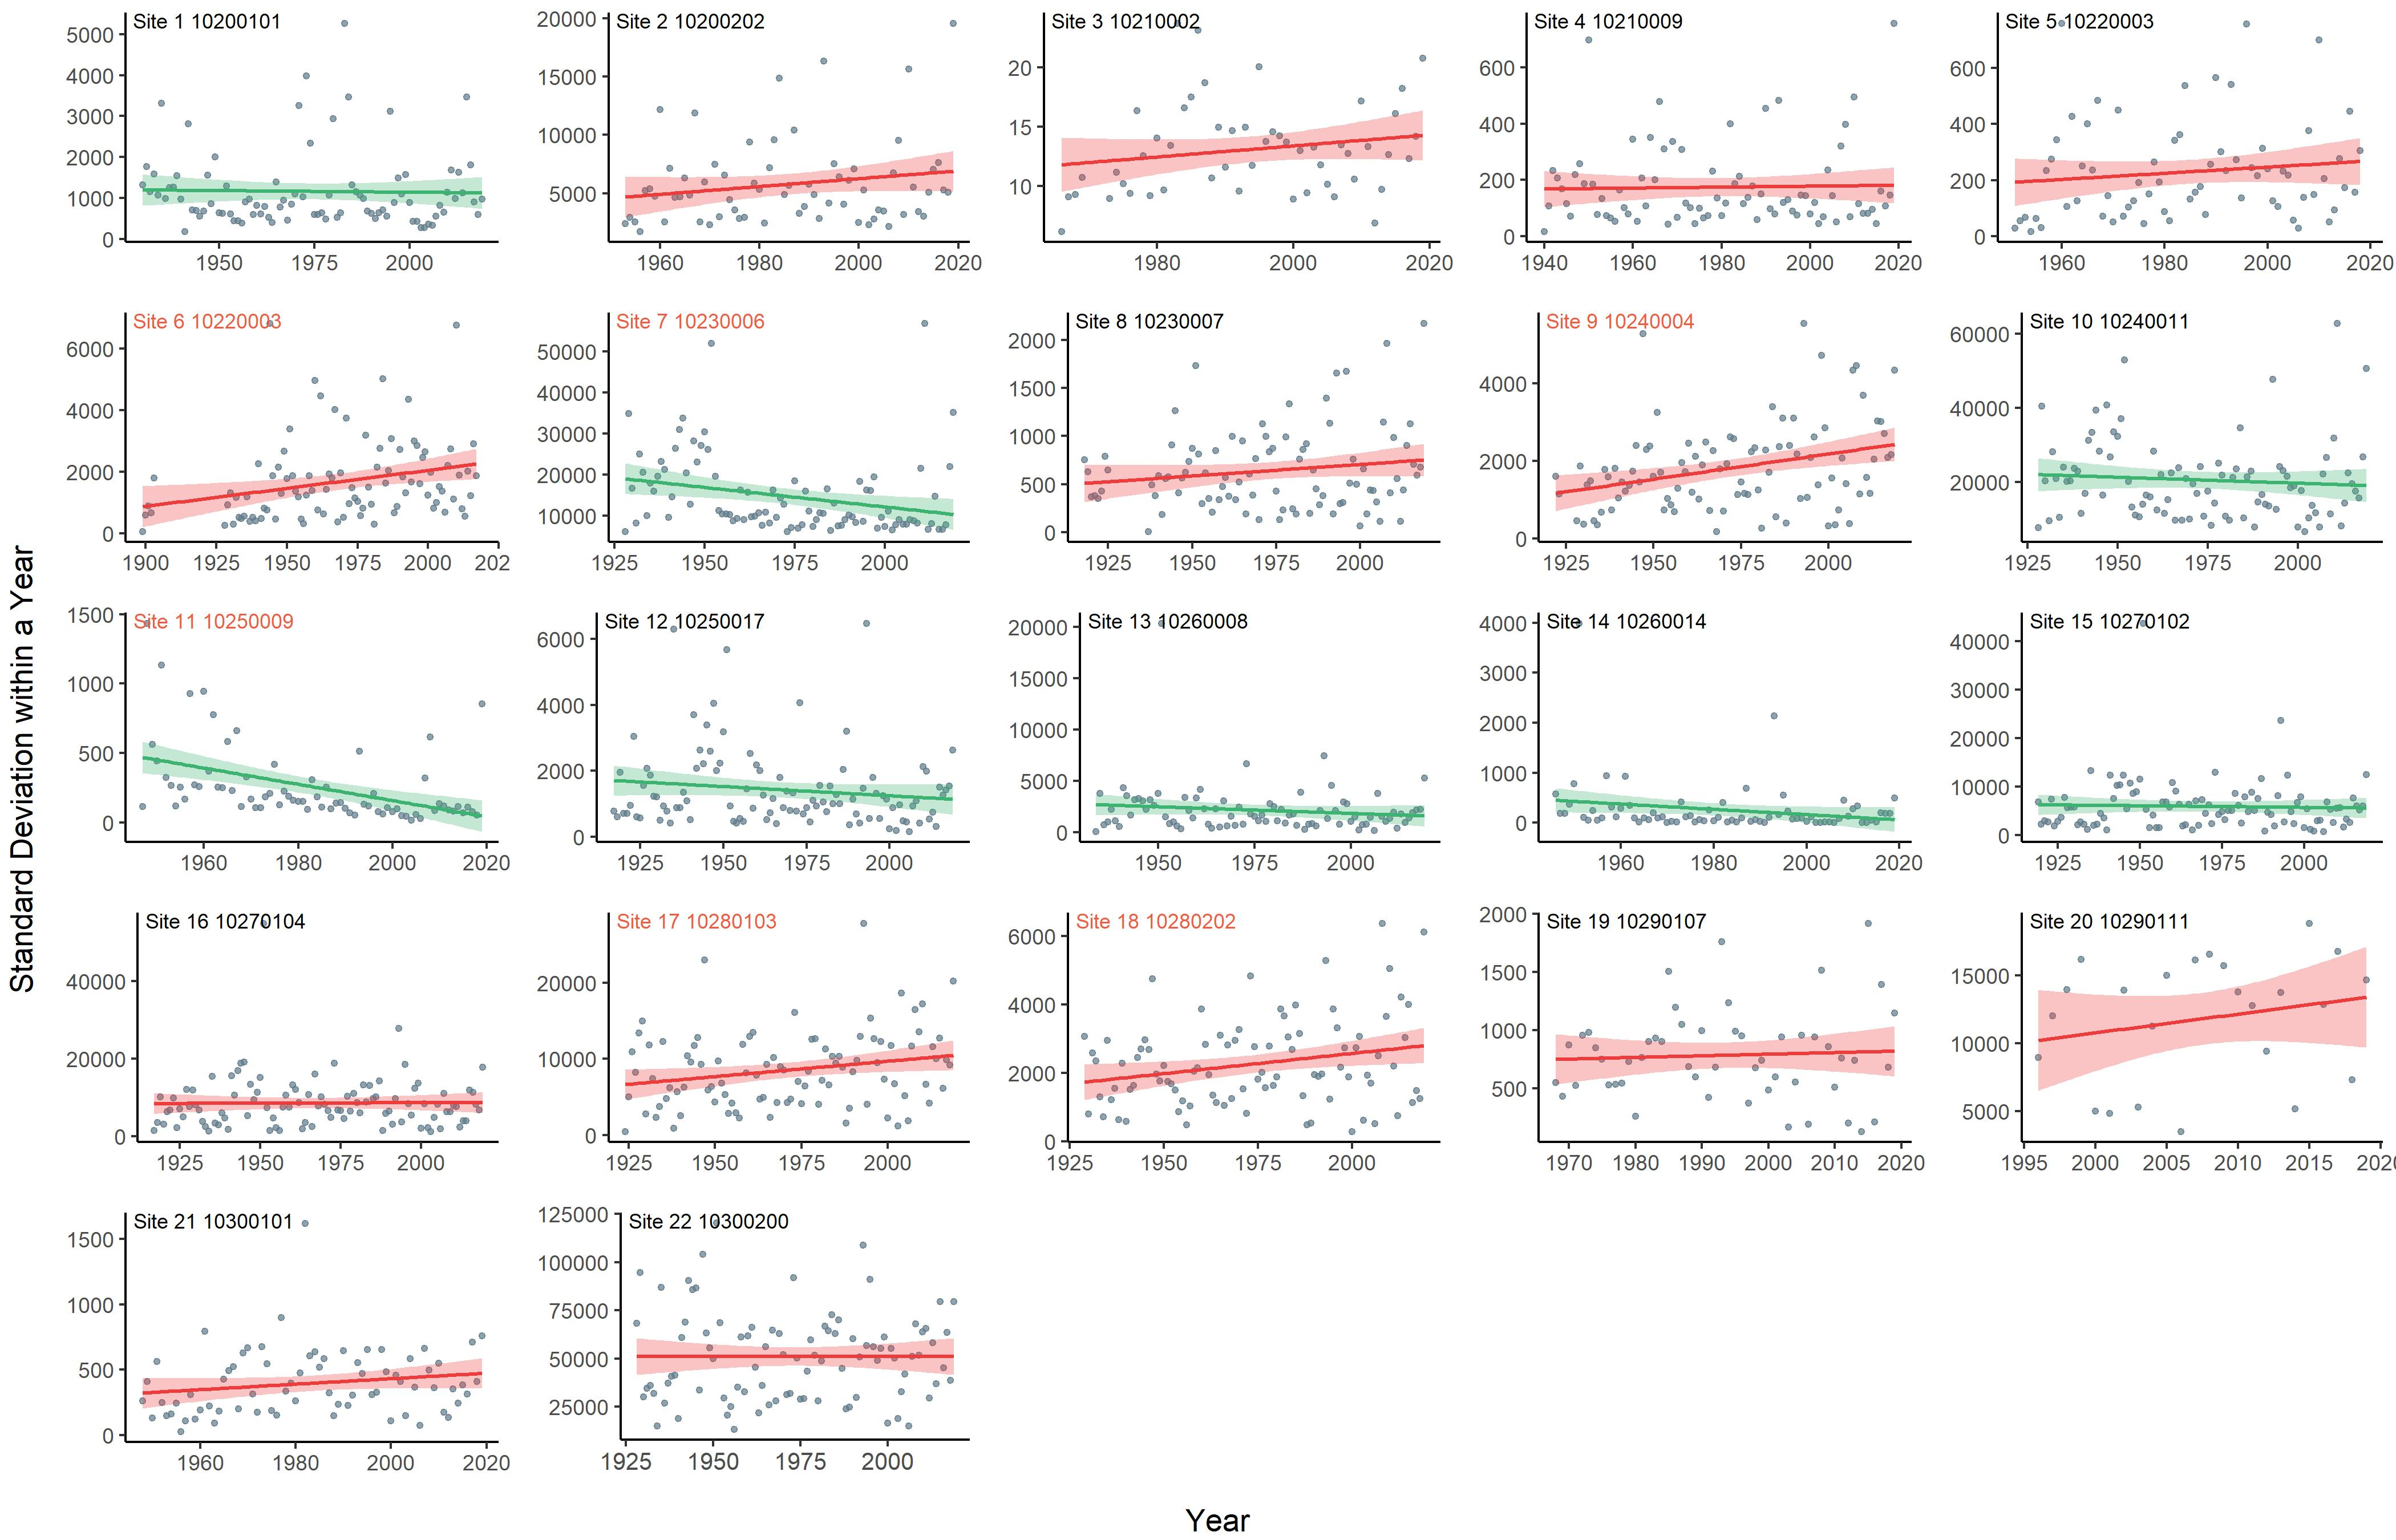
\includegraphics[width=\maxwidth]{../Figures/sd_year} \caption{\label{fig:varfig} Changes in the standard deviations (SD) of discharge within a year at 22 sites over the whole time span of available data. Red regression lines and confidence intervals suggest increasing SD, whereas blue for decreasing SD over time. Bolded site labels and HUC8 with asterisk indicate significant results, whereas regression lines in gray are non-significant ($\alpha = 0.05$).}\label{fig:varfig}
\end{figure}

\begin{table}[!h]

\caption{\label{tab:vartab}\label{tab:vartab} Slopes of linear regression between year and standard deviation or coefficient of variation of discharge at 22 sites.}
\centering
\resizebox{\linewidth}{!}{
\begin{tabular}{rcccccc}
\toprule
\multicolumn{3}{c}{ } & \multicolumn{2}{c}{Standard Deviation} & \multicolumn{2}{c}{Coefficient of Variation} \\
\cmidrule(l{3pt}r{3pt}){4-5} \cmidrule(l{3pt}r{3pt}){6-7}
No. & Site Name & HUC4 & Slope & $P$-value & Slope & $P$-value\\
\midrule
\rowcolor{gray!6}  1 & Platte River Near Overton, NE & 1020 & -0.805 & 0.004 & -0.003 & 0.004*\\
2 & Platte River At Louisville, NE & 1020 & 33.691 & 0.008 & -0.004 & 0.008*\\
\rowcolor{gray!6}  3 & Dismal River Near Thedford, NE & 1021 & 0.047 & 0.805 & 0.000 & 0.805\\
4 & Beaver Creek At Genoa, NE & 1021 & 0.168 & 0.198 & -0.004 & 0.198\\
\rowcolor{gray!6}  5 & Maple Creek Near Nickerson, NE & 1022 & 1.613 & 0.002 & -0.028 & 0.002*\\
\addlinespace
6 & Elkhorn River At Waterloo, NE & 1022 & 17.400 & 0.002** & 0.000 & 0.911\\
\rowcolor{gray!6}  7 & Missouri River At Omaha, NE & 1023 & -95.171 & 0.009** & -0.006 & 0.000***\\
8 & Boyer River At Logan, IA & 1023 & 2.404 & 0.000 & -0.012 & 0.000***\\
\rowcolor{gray!6}  9 & Nishnabotna River Above Hamburg, IA & 1024 & 13.001 & 0.002** & -0.010 & 0.000***\\
10 & Missouri River At St. Joseph, MO & 1024 & -32.123 & 0.000 & -0.004 & 0.000***\\
\addlinespace
\rowcolor{gray!6}  11 & Republican River Near Orleans, NE & 1025 & -5.861 & 0.000*** & -0.004 & 0.139\\
12 & Republican R At Clay Center, KS & 1025 & -5.579 & 0.020 & 0.004 & 0.020*\\
\rowcolor{gray!6}  13 & Smoky Hill R At Enterprise, KS & 1026 & -12.875 & 0.227 & -0.002 & 0.227\\
14 & Sf Solomon R At Osborne, KS & 1026 & -5.271 & 0.056 & -0.014 & 0.056\\
\rowcolor{gray!6}  15 & Kansas R At Wamego, KS & 1027 & -6.676 & 0.006 & -0.003 & 0.006*\\
\addlinespace
16 & Kansas R At Desoto, KS & 1027 & 2.556 & 0.007 & -0.003 & 0.007*\\
\rowcolor{gray!6}  17 & Grand River Near Sumner, MO & 1028 & 40.400 & 0.026* & 0.000 & 0.916\\
18 & Chariton River Near Prairie Hill, MO & 1028 & 11.861 & 0.020* & -0.002 & 0.200\\
\rowcolor{gray!6}  19 & Pomme De Terre River Near Polk, MO & 1029 & 1.389 & 0.798 & -0.002 & 0.798\\
20 & Osage River Below St. Thomas, MO & 1029 & 138.275 & 0.769 & -0.003 & 0.769\\
\addlinespace
\rowcolor{gray!6}  21 & Little Blue River Near Lake City, MO & 1030 & 2.096 & 0.009 & -0.012 & 0.009*\\
22 & Missouri River At Hermann, MO & 1030 & 0.657 & 0.000 & -0.003 & 0.000***\\
\bottomrule
\multicolumn{7}{l}{\textit{Note: }}\\
\multicolumn{7}{l}{Significance level}\\
\multicolumn{7}{l}{\textsuperscript{*} <0.05;}\\
\multicolumn{7}{l}{\textsuperscript{**} <0.01;}\\
\multicolumn{7}{l}{\textsuperscript{***} <0.001;}\\
\end{tabular}}
\end{table}

\newpage

\hypertarget{analysis}{%
\section{Analysis}\label{analysis}}

\textless{}Insert visualizations and text describing your main analyses.
Format your R chunks so that graphs are displayed but code and other
output is not displayed. Instead, describe the results of any
statistical tests in the main text (e.g., ``Variable x was significantly
different among y groups (ANOVA; df = 300, F = 5.55, p \textless{}
0.0001)''). Each paragraph, accompanied by one or more visualizations,
should describe the major findings and how they relate to the question
and hypotheses. Divide this section into subsections, one for each
research question.\textgreater{}

\textless{}Each figure should be accompanied by a caption, and each
figure should be referenced within the text\textgreater{}

\hypertarget{question-1-how-have-changes-in-discharge-interacted-with-nutrient-enrichment-in-the-missouri-river-basin}{%
\subsection{Question 1: How have changes in discharge interacted with
nutrient enrichment in the Missouri River
Basin?}\label{question-1-how-have-changes-in-discharge-interacted-with-nutrient-enrichment-in-the-missouri-river-basin}}

We analyzed nitrogen and phosphorus trends at 22 sites using long-term
daily value data and Seasonal Mann-Kendall Trend Test. The Seasonal Mann
Kendall Trend Test is used to analyze seasonal data collected over time
for consistently increasing or decreasing trends (monotonic) in Y
values. It is suitable for analyzing the data with seasonality,
non-parametric, no temporal autocorelation, identical distribution.

The overall results of the analysis can be seen in the following table
(Table 3).The trend of nitrogen and phosphorus concentration of 22 sites
are quite different. Among all 22 sites, 7 sites show significantly
increasing trends in nitrogen concentration, while 7 show decreasing
trends. For phosphorus, concentrations at 7 sites have increased over
time, while decreased at other 5 sites. But generally, the trend of
nitrogen and the trend of phosphorus are similar, which indicates that
there is a high possibility that nitrogen and phosphorus come from the
same sources. Despite inconsistent results at all sites, those on the
mainstem show higher nutrient concentration (No.~7 06610000 Missouri
River at Omaha, NE; No.~10 06818000 Missouri River at St.~Joseph, MO;
No.~22 06934500 Missouri River at Hermann, MO), we can see a significant
increasing trend of nitrogen and phosphorus. The water quality in
Missouri River is still deteriorating and protection is urgently needed.

\newpage

\begin{longtable}[]{@{}cccccc@{}}
\caption{Nitrogen and Phosphorus Trend over Time for Every
Site}\tabularnewline
\toprule
\begin{minipage}[b]{0.14\columnwidth}\centering
No.\strut
\end{minipage} & \begin{minipage}[b]{0.11\columnwidth}\centering
Site Number\strut
\end{minipage} & \begin{minipage}[b]{0.17\columnwidth}\centering
Nitrogen Trend\strut
\end{minipage} & \begin{minipage}[b]{0.14\columnwidth}\centering
Nitrogen Trend Significance\strut
\end{minipage} & \begin{minipage}[b]{0.11\columnwidth}\centering
Phosphorus Trend\strut
\end{minipage} & \begin{minipage}[b]{0.17\columnwidth}\centering
Phosphorus Trend Significance\strut
\end{minipage}\tabularnewline
\midrule
\endfirsthead
\toprule
\begin{minipage}[b]{0.14\columnwidth}\centering
No.\strut
\end{minipage} & \begin{minipage}[b]{0.11\columnwidth}\centering
Site Number\strut
\end{minipage} & \begin{minipage}[b]{0.17\columnwidth}\centering
Nitrogen Trend\strut
\end{minipage} & \begin{minipage}[b]{0.14\columnwidth}\centering
Nitrogen Trend Significance\strut
\end{minipage} & \begin{minipage}[b]{0.11\columnwidth}\centering
Phosphorus Trend\strut
\end{minipage} & \begin{minipage}[b]{0.17\columnwidth}\centering
Phosphorus Trend Significance\strut
\end{minipage}\tabularnewline
\midrule
\endhead
\begin{minipage}[t]{0.14\columnwidth}\centering
1\strut
\end{minipage} & \begin{minipage}[t]{0.11\columnwidth}\centering
06768000\strut
\end{minipage} & \begin{minipage}[t]{0.17\columnwidth}\centering
Decrease\strut
\end{minipage} & \begin{minipage}[t]{0.14\columnwidth}\centering
*\strut
\end{minipage} & \begin{minipage}[t]{0.11\columnwidth}\centering
Decrease\strut
\end{minipage} & \begin{minipage}[t]{0.17\columnwidth}\centering
***\strut
\end{minipage}\tabularnewline
\begin{minipage}[t]{0.14\columnwidth}\centering
2\strut
\end{minipage} & \begin{minipage}[t]{0.11\columnwidth}\centering
06805500\strut
\end{minipage} & \begin{minipage}[t]{0.17\columnwidth}\centering
Increase\strut
\end{minipage} & \begin{minipage}[t]{0.14\columnwidth}\centering
***\strut
\end{minipage} & \begin{minipage}[t]{0.11\columnwidth}\centering
Increase\strut
\end{minipage} & \begin{minipage}[t]{0.17\columnwidth}\centering
***\strut
\end{minipage}\tabularnewline
\begin{minipage}[t]{0.14\columnwidth}\centering
3\strut
\end{minipage} & \begin{minipage}[t]{0.11\columnwidth}\centering
06775900\strut
\end{minipage} & \begin{minipage}[t]{0.17\columnwidth}\centering
Decrease\strut
\end{minipage} & \begin{minipage}[t]{0.14\columnwidth}\centering
***\strut
\end{minipage} & \begin{minipage}[t]{0.11\columnwidth}\centering
Decrease\strut
\end{minipage} & \begin{minipage}[t]{0.17\columnwidth}\centering
\strut
\end{minipage}\tabularnewline
\begin{minipage}[t]{0.14\columnwidth}\centering
4\strut
\end{minipage} & \begin{minipage}[t]{0.11\columnwidth}\centering
06794000\strut
\end{minipage} & \begin{minipage}[t]{0.17\columnwidth}\centering
Increase\strut
\end{minipage} & \begin{minipage}[t]{0.14\columnwidth}\centering
\strut
\end{minipage} & \begin{minipage}[t]{0.11\columnwidth}\centering
Increase\strut
\end{minipage} & \begin{minipage}[t]{0.17\columnwidth}\centering
\strut
\end{minipage}\tabularnewline
\begin{minipage}[t]{0.14\columnwidth}\centering
5\strut
\end{minipage} & \begin{minipage}[t]{0.11\columnwidth}\centering
06800000\strut
\end{minipage} & \begin{minipage}[t]{0.17\columnwidth}\centering
Increase\strut
\end{minipage} & \begin{minipage}[t]{0.14\columnwidth}\centering
***\strut
\end{minipage} & \begin{minipage}[t]{0.11\columnwidth}\centering
Increase\strut
\end{minipage} & \begin{minipage}[t]{0.17\columnwidth}\centering
***\strut
\end{minipage}\tabularnewline
\begin{minipage}[t]{0.14\columnwidth}\centering
6\strut
\end{minipage} & \begin{minipage}[t]{0.11\columnwidth}\centering
06800500\strut
\end{minipage} & \begin{minipage}[t]{0.17\columnwidth}\centering
Increase\strut
\end{minipage} & \begin{minipage}[t]{0.14\columnwidth}\centering
*\strut
\end{minipage} & \begin{minipage}[t]{0.11\columnwidth}\centering
Increase\strut
\end{minipage} & \begin{minipage}[t]{0.17\columnwidth}\centering
\strut
\end{minipage}\tabularnewline
\begin{minipage}[t]{0.14\columnwidth}\centering
7\strut
\end{minipage} & \begin{minipage}[t]{0.11\columnwidth}\centering
06610000\strut
\end{minipage} & \begin{minipage}[t]{0.17\columnwidth}\centering
Increase\strut
\end{minipage} & \begin{minipage}[t]{0.14\columnwidth}\centering
**\strut
\end{minipage} & \begin{minipage}[t]{0.11\columnwidth}\centering
Increase\strut
\end{minipage} & \begin{minipage}[t]{0.17\columnwidth}\centering
***\strut
\end{minipage}\tabularnewline
\begin{minipage}[t]{0.14\columnwidth}\centering
8\strut
\end{minipage} & \begin{minipage}[t]{0.11\columnwidth}\centering
06609500\strut
\end{minipage} & \begin{minipage}[t]{0.17\columnwidth}\centering
Decrease\strut
\end{minipage} & \begin{minipage}[t]{0.14\columnwidth}\centering
\strut
\end{minipage} & \begin{minipage}[t]{0.11\columnwidth}\centering
Increase\strut
\end{minipage} & \begin{minipage}[t]{0.17\columnwidth}\centering
\strut
\end{minipage}\tabularnewline
\begin{minipage}[t]{0.14\columnwidth}\centering
9\strut
\end{minipage} & \begin{minipage}[t]{0.11\columnwidth}\centering
06810000\strut
\end{minipage} & \begin{minipage}[t]{0.17\columnwidth}\centering
Decrease\strut
\end{minipage} & \begin{minipage}[t]{0.14\columnwidth}\centering
\strut
\end{minipage} & \begin{minipage}[t]{0.11\columnwidth}\centering
Increase\strut
\end{minipage} & \begin{minipage}[t]{0.17\columnwidth}\centering
\strut
\end{minipage}\tabularnewline
\begin{minipage}[t]{0.14\columnwidth}\centering
10\strut
\end{minipage} & \begin{minipage}[t]{0.11\columnwidth}\centering
06818000\strut
\end{minipage} & \begin{minipage}[t]{0.17\columnwidth}\centering
Increase\strut
\end{minipage} & \begin{minipage}[t]{0.14\columnwidth}\centering
.\strut
\end{minipage} & \begin{minipage}[t]{0.11\columnwidth}\centering
Increase\strut
\end{minipage} & \begin{minipage}[t]{0.17\columnwidth}\centering
\strut
\end{minipage}\tabularnewline
\begin{minipage}[t]{0.14\columnwidth}\centering
11\strut
\end{minipage} & \begin{minipage}[t]{0.11\columnwidth}\centering
06844500\strut
\end{minipage} & \begin{minipage}[t]{0.17\columnwidth}\centering
Increase\strut
\end{minipage} & \begin{minipage}[t]{0.14\columnwidth}\centering
.\strut
\end{minipage} & \begin{minipage}[t]{0.11\columnwidth}\centering
Decrease\strut
\end{minipage} & \begin{minipage}[t]{0.17\columnwidth}\centering
**\strut
\end{minipage}\tabularnewline
\begin{minipage}[t]{0.14\columnwidth}\centering
12\strut
\end{minipage} & \begin{minipage}[t]{0.11\columnwidth}\centering
06856600\strut
\end{minipage} & \begin{minipage}[t]{0.17\columnwidth}\centering
Decrease\strut
\end{minipage} & \begin{minipage}[t]{0.14\columnwidth}\centering
**\strut
\end{minipage} & \begin{minipage}[t]{0.11\columnwidth}\centering
Decrease\strut
\end{minipage} & \begin{minipage}[t]{0.17\columnwidth}\centering
***\strut
\end{minipage}\tabularnewline
\begin{minipage}[t]{0.14\columnwidth}\centering
13\strut
\end{minipage} & \begin{minipage}[t]{0.11\columnwidth}\centering
06877600\strut
\end{minipage} & \begin{minipage}[t]{0.17\columnwidth}\centering
Decrease\strut
\end{minipage} & \begin{minipage}[t]{0.14\columnwidth}\centering
.\strut
\end{minipage} & \begin{minipage}[t]{0.11\columnwidth}\centering
Increase\strut
\end{minipage} & \begin{minipage}[t]{0.17\columnwidth}\centering
\strut
\end{minipage}\tabularnewline
\begin{minipage}[t]{0.14\columnwidth}\centering
14\strut
\end{minipage} & \begin{minipage}[t]{0.11\columnwidth}\centering
06874000\strut
\end{minipage} & \begin{minipage}[t]{0.17\columnwidth}\centering
Decrease\strut
\end{minipage} & \begin{minipage}[t]{0.14\columnwidth}\centering
***\strut
\end{minipage} & \begin{minipage}[t]{0.11\columnwidth}\centering
Decrease\strut
\end{minipage} & \begin{minipage}[t]{0.17\columnwidth}\centering
***\strut
\end{minipage}\tabularnewline
\begin{minipage}[t]{0.14\columnwidth}\centering
15\strut
\end{minipage} & \begin{minipage}[t]{0.11\columnwidth}\centering
06887500\strut
\end{minipage} & \begin{minipage}[t]{0.17\columnwidth}\centering
Increase\strut
\end{minipage} & \begin{minipage}[t]{0.14\columnwidth}\centering
***\strut
\end{minipage} & \begin{minipage}[t]{0.11\columnwidth}\centering
Increase\strut
\end{minipage} & \begin{minipage}[t]{0.17\columnwidth}\centering
***\strut
\end{minipage}\tabularnewline
\begin{minipage}[t]{0.14\columnwidth}\centering
16\strut
\end{minipage} & \begin{minipage}[t]{0.11\columnwidth}\centering
06892350\strut
\end{minipage} & \begin{minipage}[t]{0.17\columnwidth}\centering
Increase\strut
\end{minipage} & \begin{minipage}[t]{0.14\columnwidth}\centering
**\strut
\end{minipage} & \begin{minipage}[t]{0.11\columnwidth}\centering
Increase\strut
\end{minipage} & \begin{minipage}[t]{0.17\columnwidth}\centering
***\strut
\end{minipage}\tabularnewline
\begin{minipage}[t]{0.14\columnwidth}\centering
17\strut
\end{minipage} & \begin{minipage}[t]{0.11\columnwidth}\centering
06902000\strut
\end{minipage} & \begin{minipage}[t]{0.17\columnwidth}\centering
Decrease\strut
\end{minipage} & \begin{minipage}[t]{0.14\columnwidth}\centering
***\strut
\end{minipage} & \begin{minipage}[t]{0.11\columnwidth}\centering
Increase\strut
\end{minipage} & \begin{minipage}[t]{0.17\columnwidth}\centering
\strut
\end{minipage}\tabularnewline
\begin{minipage}[t]{0.14\columnwidth}\centering
18\strut
\end{minipage} & \begin{minipage}[t]{0.11\columnwidth}\centering
06905500\strut
\end{minipage} & \begin{minipage}[t]{0.17\columnwidth}\centering
Decrease\strut
\end{minipage} & \begin{minipage}[t]{0.14\columnwidth}\centering
\strut
\end{minipage} & \begin{minipage}[t]{0.11\columnwidth}\centering
Increase\strut
\end{minipage} & \begin{minipage}[t]{0.17\columnwidth}\centering
\strut
\end{minipage}\tabularnewline
\begin{minipage}[t]{0.14\columnwidth}\centering
19\strut
\end{minipage} & \begin{minipage}[t]{0.11\columnwidth}\centering
06921070\strut
\end{minipage} & \begin{minipage}[t]{0.17\columnwidth}\centering
Decrease\strut
\end{minipage} & \begin{minipage}[t]{0.14\columnwidth}\centering
.\strut
\end{minipage} & \begin{minipage}[t]{0.11\columnwidth}\centering
Decrease\strut
\end{minipage} & \begin{minipage}[t]{0.17\columnwidth}\centering
\strut
\end{minipage}\tabularnewline
\begin{minipage}[t]{0.14\columnwidth}\centering
20\strut
\end{minipage} & \begin{minipage}[t]{0.11\columnwidth}\centering
06926510\strut
\end{minipage} & \begin{minipage}[t]{0.17\columnwidth}\centering
Decrease\strut
\end{minipage} & \begin{minipage}[t]{0.14\columnwidth}\centering
***\strut
\end{minipage} & \begin{minipage}[t]{0.11\columnwidth}\centering
Increase\strut
\end{minipage} & \begin{minipage}[t]{0.17\columnwidth}\centering
***\strut
\end{minipage}\tabularnewline
\begin{minipage}[t]{0.14\columnwidth}\centering
21\strut
\end{minipage} & \begin{minipage}[t]{0.11\columnwidth}\centering
06894000\strut
\end{minipage} & \begin{minipage}[t]{0.17\columnwidth}\centering
Decrease\strut
\end{minipage} & \begin{minipage}[t]{0.14\columnwidth}\centering
***\strut
\end{minipage} & \begin{minipage}[t]{0.11\columnwidth}\centering
Decrease\strut
\end{minipage} & \begin{minipage}[t]{0.17\columnwidth}\centering
***\strut
\end{minipage}\tabularnewline
\begin{minipage}[t]{0.14\columnwidth}\centering
22\strut
\end{minipage} & \begin{minipage}[t]{0.11\columnwidth}\centering
06934500\strut
\end{minipage} & \begin{minipage}[t]{0.17\columnwidth}\centering
Increase\strut
\end{minipage} & \begin{minipage}[t]{0.14\columnwidth}\centering
***\strut
\end{minipage} & \begin{minipage}[t]{0.11\columnwidth}\centering
Increase\strut
\end{minipage} & \begin{minipage}[t]{0.17\columnwidth}\centering
***\strut
\end{minipage}\tabularnewline
\bottomrule
\end{longtable}

Note:

'***' p-value \textless{} 0.001

'**' 0.001 ≤ p-value \textless{} 0.01

'*' 0.01 \textless{}= p-value \textless{} 0.05

`.' 0.05 \textless{}= p-value \textless{} 0.1

otherwise 0.1 \textless{}= p-value \textless{} 1

In order to determine whether nutrient levels increase with discharge,
C-Q (concentration - discharge) plots were created for each site
(\autoref{fig:CQplot}). At sites with high frequency nitrogen data, high
frequency nitrogen and discharge values were used. When sites did not
have high frequency nitrogen data, daily values were used. A linear
model with total nitrogen as the response variable and discharge as the
independent variable was created for every site to determine if there
was a linear relationship between the two. In 18 out of 22 total sites,
there was a significant relationship where as discharge increased,
nitrogen also increased (p \textless{} 0.05).

\begin{figure}[H]
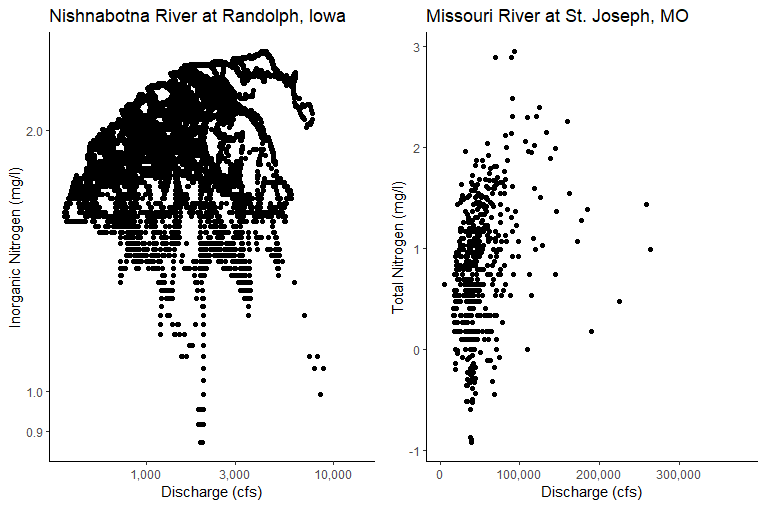
\includegraphics[width=\maxwidth]{../Figures/CQplots} \caption{\label{fig:CQplot} C-Q plots of two sites in the Missouri River Basin. High frequency (left) and daily values (right) shown for two different sites. Nitrogen values are log transformed.}\label{fig:CQplot}
\end{figure}

\hypertarget{question-2-what-effects-do-specific-flood-and-drought-events-have-on-the-water-quality-and-quantity-of-rivers-in-the-missouri-river-basin-areas-of-interest}{%
\subsection{Question 2: What effects do specific flood and drought
events have on the water quality and quantity of rivers in the Missouri
River Basin areas of
interest?}\label{question-2-what-effects-do-specific-flood-and-drought-events-have-on-the-water-quality-and-quantity-of-rivers-in-the-missouri-river-basin-areas-of-interest}}

\hypertarget{flooding}{%
\subsubsection{Flooding}\label{flooding}}

Population of each county (from the 2010 census) in the four states that
make up our region area of interest (Kansas, Nebraska, Missouri, and
Iowa) were found using the ``counties'' database from R's
\texttt{noncensus} package. We decided that population could be used as
a proxy for land cover, as a greater population would indicate more
development and fewer agricultural fields or open spaces.

Baseflow and quickflow from each site were determined with the
\texttt{EcoHydRology} package. After linearly interpolating the
instantaneous discharge data in order to account for gaps, total
baseflow volume was found and the percent of discharge exported as
baseflow was calculated. We predicted that a site within a county with a
large population would have a lower percent of its discharge exported as
baseflow, because quickflow would be more common in areas with a lot of
development. Similarly, we also predicted that a site within a county
with a small population would have a greater percentage of its discharge
coming from baseflow. More developed areas often have flashier floods,
and so we were curious to see whether we can relate population to an
element of flashiness - the percentage of discharge exported as
quickflow.

Contrary to our hypotheses, greater county population does not
contribute to a decrease in percent of discharge as baseflow (p =
0.4199, F = 0.8067) in our sites of interest. This may be due to our
small sample size of sites, or perhaps the size of the rivers in our
study.

High frequency nitrogen data was only available for six sites within our
region. In order to better understand the behavior of rivers during
floods, we examined dygraph plots of discharge and nitrogen, and created
hysteresis plots. Storms from the fall of 2018 (September - December)
were examined for each river site with data from that time period. We
chose to only look at storms that occurred in the second half of the
year in order to avoid conflating snowpack melt and precipitation
affects.

We predicted that most rivers in the area would behave the same way, and
that rivers would exhibit flushing behavior. We thought that flushing
rivers would be more prevalent because of the many agricultural fields
in our region of study, and any overland flow to the rivers would bring
with it a high concentration of nutrients (nitrogen being one of them)
from the fertilized fields. Our results say otherwise (Table 4). Our
sites of interest had both positive and negative slopes in the
hysteresis plots, and also exhibited both clockwise and counter
clockwise directions of flow (\autoref{fig:Randolphstorm}). The same
river was analyzed multiple times throughout the year, and even the same
river showed different slopes and directions in the hysteresis plots for
different storm events.

\begin{figure}
\centering
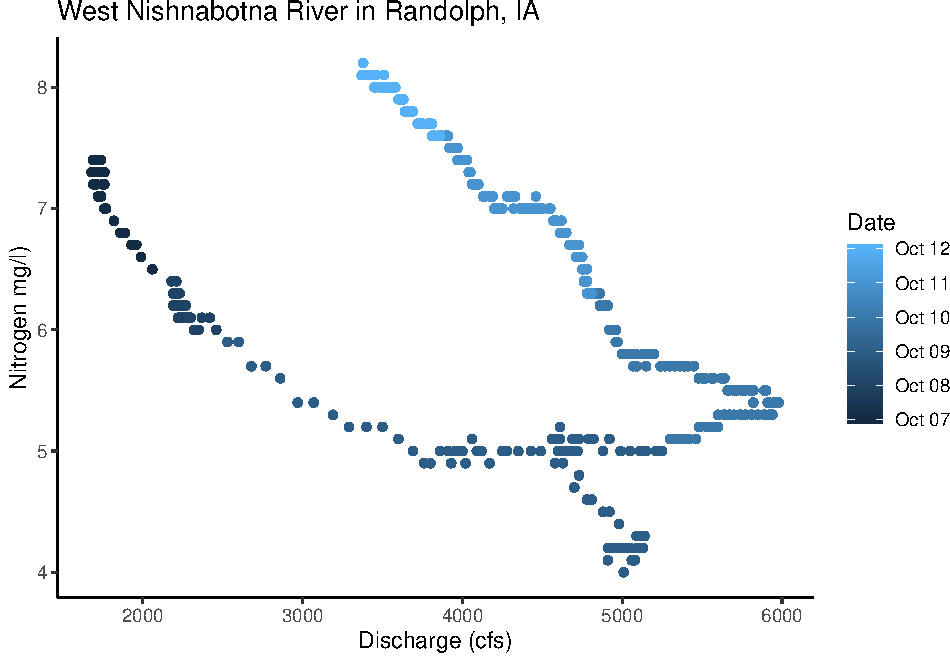
\includegraphics{Missouri-Reasearch-Project---FINAL_files/figure-latex/Randolphstorm-1.pdf}
\caption{\label{fig:Randolphstorm}Hyteresis plot for site in Randolph,
IA that shows a negative slope (diluting behavior) in a counter
clockwise direction.}
\end{figure}

\begin{longtable}[]{@{}lclll@{}}
\caption{XXX}\tabularnewline
\toprule
\begin{minipage}[b]{0.15\columnwidth}\raggedright
Site Name\strut
\end{minipage} & \begin{minipage}[b]{0.22\columnwidth}\centering
Site Number\strut
\end{minipage} & \begin{minipage}[b]{0.20\columnwidth}\raggedright
Time Period\strut
\end{minipage} & \begin{minipage}[b]{0.17\columnwidth}\raggedright
Direction\strut
\end{minipage} & \begin{minipage}[b]{0.12\columnwidth}\raggedright
Slope\strut
\end{minipage}\tabularnewline
\midrule
\endfirsthead
\toprule
\begin{minipage}[b]{0.15\columnwidth}\raggedright
Site Name\strut
\end{minipage} & \begin{minipage}[b]{0.22\columnwidth}\centering
Site Number\strut
\end{minipage} & \begin{minipage}[b]{0.20\columnwidth}\raggedright
Time Period\strut
\end{minipage} & \begin{minipage}[b]{0.17\columnwidth}\raggedright
Direction\strut
\end{minipage} & \begin{minipage}[b]{0.12\columnwidth}\raggedright
Slope\strut
\end{minipage}\tabularnewline
\midrule
\endhead
\begin{minipage}[t]{0.15\columnwidth}\raggedright
West Nishnabotna River in Randolph, IA\strut
\end{minipage} & \begin{minipage}[t]{0.22\columnwidth}\centering
06808500\strut
\end{minipage} & \begin{minipage}[t]{0.20\columnwidth}\raggedright
Oct 7 - 13, 2018\strut
\end{minipage} & \begin{minipage}[t]{0.17\columnwidth}\raggedright
counter clockwise\strut
\end{minipage} & \begin{minipage}[t]{0.12\columnwidth}\raggedright
negative (\autoref{fig:Randolphstorm})\strut
\end{minipage}\tabularnewline
\begin{minipage}[t]{0.15\columnwidth}\raggedright
Nodaway River at Clarinda, IA\strut
\end{minipage} & \begin{minipage}[t]{0.22\columnwidth}\centering
06817000\strut
\end{minipage} & \begin{minipage}[t]{0.20\columnwidth}\raggedright
Oct 8 - 12, 2018\strut
\end{minipage} & \begin{minipage}[t]{0.17\columnwidth}\raggedright
clockwise\strut
\end{minipage} & \begin{minipage}[t]{0.12\columnwidth}\raggedright
negative\strut
\end{minipage}\tabularnewline
\begin{minipage}[t]{0.15\columnwidth}\raggedright
Kansas River in Desoto, KS\strut
\end{minipage} & \begin{minipage}[t]{0.22\columnwidth}\centering
06892350\strut
\end{minipage} & \begin{minipage}[t]{0.20\columnwidth}\raggedright
Nov 30 - Dec 5, 2018\strut
\end{minipage} & \begin{minipage}[t]{0.17\columnwidth}\raggedright
counter clockwise\strut
\end{minipage} & \begin{minipage}[t]{0.12\columnwidth}\raggedright
positive\strut
\end{minipage}\tabularnewline
\begin{minipage}[t]{0.15\columnwidth}\raggedright
Missouri River at Hermann, MO\strut
\end{minipage} & \begin{minipage}[t]{0.22\columnwidth}\centering
06934500\strut
\end{minipage} & \begin{minipage}[t]{0.20\columnwidth}\raggedright
Oct 7 - 20, 2018\strut
\end{minipage} & \begin{minipage}[t]{0.17\columnwidth}\raggedright
counter clockwise\strut
\end{minipage} & \begin{minipage}[t]{0.12\columnwidth}\raggedright
negative\strut
\end{minipage}\tabularnewline
\begin{minipage}[t]{0.15\columnwidth}\raggedright
Mill C at Johnson Drive, Shawnee, KS\strut
\end{minipage} & \begin{minipage}[t]{0.22\columnwidth}\centering
06892513\strut
\end{minipage} & \begin{minipage}[t]{0.20\columnwidth}\raggedright
Nov 27 - Dec 4, 2018\strut
\end{minipage} & \begin{minipage}[t]{0.17\columnwidth}\raggedright
clockwise\strut
\end{minipage} & \begin{minipage}[t]{0.12\columnwidth}\raggedright
negative\strut
\end{minipage}\tabularnewline
\begin{minipage}[t]{0.15\columnwidth}\raggedright
Grand River, Sumner MO\strut
\end{minipage} & \begin{minipage}[t]{0.22\columnwidth}\centering
06902000\strut
\end{minipage} & \begin{minipage}[t]{0.20\columnwidth}\raggedright
Sep 6 - 10, 2018\strut
\end{minipage} & \begin{minipage}[t]{0.17\columnwidth}\raggedright
clockwise\strut
\end{minipage} & \begin{minipage}[t]{0.12\columnwidth}\raggedright
positive\strut
\end{minipage}\tabularnewline
\bottomrule
\end{longtable}

\hypertarget{droughts}{%
\subsubsection{Droughts}\label{droughts}}

Droughts in the Missouri River Basin were known to occur throughout the
years and six sites were analyzed for drought information. The six sites
were chosen based off what was examined for floods.

Drought was defined as determining the 7Q10, which is the minimum 7-day
average flow that will occur every 10 years (probability of 10\%) (EPA,
2019). The 7Q10 measurement is used to determine streamflow limits,
allocate water resources, dilution rates in watersheds, and more (USGS,
2019). 7Q10 is calculated by determining the recurrence interval, which
is the past recurrence of an event, which for droughts would be the
minimum 7-day average discharge. The recurrence interval can then be
used to calculate the probability, which would be the probability or
likelihood of having a minimum 7-day average flow of this magnitude or
greater. In this case, the minimum 7-day average flow that has a 10\%
chance of going below that value in a given year.

The recurrence interval is calculated using the following equation:

\[T = (n+1)/m\]

where T is the recurrence interval, n is the number of years of data,
and m is the ranking of the event within the years of data.

Exceedance probability is calculated to determine the probability of
having a discharge event of a given size or greater in a year. The
equation is:

\[P = 1/T\]

where P is the exceedance probability, and T is the recurrence interval.

The 7Q10 was calculated for each of the six sites by first filtering the
discharge data to only include the selected site. The `rollmean'
function was then used to calculate the average flow every 7 days for
said site. Once the 7-day average flow was calculated, the data was
grouped by the year so that it could then be summarized to obtain the
minimum 7-day average flow. After grouping and summarizing the data,
there was one value, the minimum 7-day average flow, for each year of
data obtained. From here, the recurrence interval and probability were
calculated in each data frame.

The miniumum 7 day average flow (cfs) for each river differed and the
miniumum 7 day average low flow (cfs) varied from year to year in the
same river (\autoref{fig:MinFlowMill}).

\begin{figure}
\centering
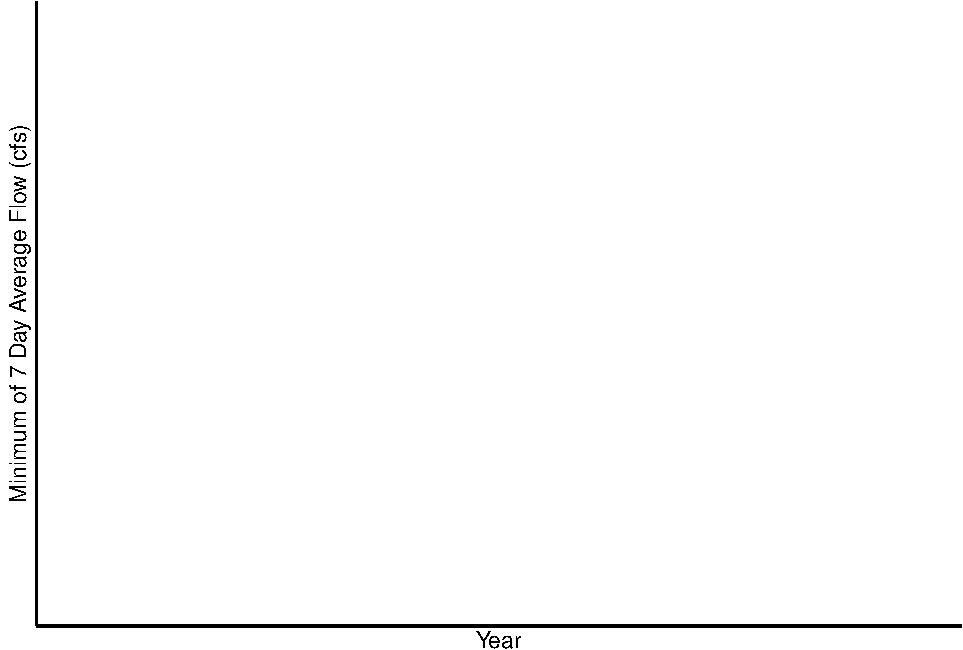
\includegraphics{Missouri-Reasearch-Project---FINAL_files/figure-latex/MinFlowMill-1.pdf}
\caption{\label{fig:MinFlowMill}Plot showing the minimum 7 day average
flow (cfs) at Mill Creek for the period of record (October 2002 -
November 2019). The miniumum 7 day average flow was very low in 2012 and
decreased again in 2018.}
\end{figure}

The 7Q10 value was then determined from the probability column by
filtering the data to show the minimum 7-day average discharge with
probability less than or equal to 0.1 (Table 3).

\begin{longtable}[]{@{}lll@{}}
\caption{WRITE caption summarizing the 7Q10 values for each of the
streams that were analyzed for droughts.}\tabularnewline
\toprule
Site Name & Site Number & 7Q10 Minimum Discharge (cfs)\tabularnewline
\midrule
\endfirsthead
\toprule
Site Name & Site Number & 7Q10 Minimum Discharge (cfs)\tabularnewline
\midrule
\endhead
West Nishnabotna River in Randolph, IA & 06808500 & 41.3\tabularnewline
Nodaway River at Clarinda, IA & 06817000 & 5.93\tabularnewline
Kansas River in Desoto, KS & 06892350 & 562\tabularnewline
Missouri River at Hermann, MO & 06934500 & 12414\tabularnewline
Mill C at Johnson Drive, Shawnee, KS & 06892513 & 1.47\tabularnewline
Grand River, Sumner MO & 06902000 & 39.1\tabularnewline
\bottomrule
\end{longtable}

In addition to calculating the 7Q10 values for the 6 sites, the sites
were analyzed to determine the 30-day moving average flow over a period
of years. This was done using code from USGS to calculate moving
averages and historical quantiles (USGS, 2016). The 25th, 50th, and 75th
quantiles were calculated to determine the minimum, median, and maximum
values for discharge in a given year to determine historical flow. The
30-day moving average flow over a period of years was then plotted with
Normal (25th to 75th percentile), Drought Watch (10th to 25th
percentile), Drought Warning (5th to 10th percentile), and Drought
Emergency (0 to 5th percentile) (\autoref{fig:Milldrought}). This
information about what flow would constitute a drought is extremely
useful for water managers.

<<<<<<< HEAD
\begin{verbatim}
## 
##    1    2 
## 6257    1
\end{verbatim}

\includegraphics{Missouri-Reasearch-Project---FINAL_files/figure-latex/Milldrought-1.pdf}
\includegraphics{Missouri-Reasearch-Project---FINAL_files/figure-latex/Milldrought-2.pdf}

=======
>>>>>>> 5d321b88819c6cf0c8ae22b21efafc6a4c9de8b3
\hypertarget{question-3-what-factors-contribute-to-the-variability-of-total-nitrogen-in-the-rivers}{%
\subsection{Question 3: What factors contribute to the variability of
total nitrogen in the
rivers?}\label{question-3-what-factors-contribute-to-the-variability-of-total-nitrogen-in-the-rivers}}

In order to better understand what contributes to the variability of
nitrogen concentration in our study area of interest, we created a
linear model with fixed effects and random effects. By considering the
HUC 4 region each site is in as a random effect, we can estimate the
amount of variation of nitrogen between each HUC 4. In order to better
model the interaction, I chose to divide the year variable by 10 and the
population by 1000 so that rescaling is not an issue. The model chosen
is below:

\begin{quote}
\texttt{lmer(data,\ log(total.nitrogen)\ \textasciitilde{}\ Year\ +\ population\ \ +\ (1\textbar{}huc4))}
\end{quote}

Year and population are fixed effects while the grouping of the HUC 4
region is a random effect. This means we take the HUC 4 region variance
into account when modeling the effect of year and population on total
nitrogen. Using log transformed nitrogen data and HUC 4 region as a
random effect, there is a significant difference in total nitrogen
across each decade and every 1000 people (p \textless{} 2e-16). The
regression equation is below:

\[log(Total Nitrogen) = -3.68 + 0.0229(Year/10) - 9.95e-04(population/1000)\]

Because we used a log transformed data set, we have to exponentiate the
coefficients in the model to interpret them. The intercept is 0.025,
which is the mean of total nitrogen when year is 0 and population is 0.
When exponentiating the Year coefficient, we can conclude that every
decade has a 1.02 multiplicative effect on nitrogen. When exponentiating
the population coefficient, we can conclude that every 1000 people have
a 0.99 multiplicative effect on nitrogen. The model demonstrates the the
level of decade and population affected the total nitrogen in each HUC 4
region. Residuals are evenly distributed, and the R\^{}2 value = 0.514,
indicating that 51.4\% of the variation in nitrogen is explained by this
model.

\hypertarget{question-4-given-past-and-current-data-what-can-we-predict-about-the-future-state-of-water-in-the-missouri-river-basin}{%
\subsection{Question 4: Given past and current data, what can we predict
about the future state of water in the Missouri River
Basin?}\label{question-4-given-past-and-current-data-what-can-we-predict-about-the-future-state-of-water-in-the-missouri-river-basin}}

\hypertarget{discharge-trends-analysis}{%
\subsubsection{Discharge Trends
Analysis}\label{discharge-trends-analysis}}

We also analyzed discharge trend at 22 sites using daily value data and
Mann-Kandall Trend Test. The results are listed in the following table
(Table 6). In our analysis, discharge of 18 sites increases while 4
sites show the decreasing trend of discharge. However, these four sites
all locate in HUC 1025 and 1026, away from the main stem of the Missouri
River. Therefore, overall, the discharge in Missouri River is
increasing.

\newpage

\begin{longtable}[]{@{}cccc@{}}
\caption{Discharge Trend over Time}\tabularnewline
\toprule
NO. & Site Number & Discharge Trend & Discharge Trend
Significance\tabularnewline
\midrule
\endfirsthead
\toprule
NO. & Site Number & Discharge Trend & Discharge Trend
Significance\tabularnewline
\midrule
\endhead
1 & 06768000 & Increase &\tabularnewline
2 & 06805500 & Increase & ***\tabularnewline
3 & 06775900 & Increase & ***\tabularnewline
4 & 06794000 & Increase &\tabularnewline
5 & 06800000 & Increase & ***\tabularnewline
6 & 06800500 & Increase & ***\tabularnewline
7 & 06610000 & Increase & ***\tabularnewline
8 & 06609500 & Increase & ***\tabularnewline
9 & 06810000 & Increase & ***\tabularnewline
10 & 06818000 & Increase & ***\tabularnewline
11 & 06844500 & Decrease & ***\tabularnewline
12 & 06856600 & Decrease & **\tabularnewline
13 & 06877600 & Decrease &\tabularnewline
14 & 06874000 & Decrease & .\tabularnewline
15 & 06887500 & Increase &\tabularnewline
16 & 06892350 & Increase & .\tabularnewline
17 & 06902000 & Increase & *\tabularnewline
18 & 06905500 & Increase & *\tabularnewline
19 & 06921070 & Increase &\tabularnewline
20 & 06926510 & Increase &\tabularnewline
21 & 06894000 & Increase & **\tabularnewline
22 & 06934500 & Increase & ***\tabularnewline
\bottomrule
\end{longtable}

Note:

'***' p-value \textless{} 0.001

'**' 0.001 \textless{}= p-value \textless{} 0.01

'*' 0.01 \textless{}= p-value \textless{} 0.05

`.' 0.05 \textless{}= p-value \textless{} 0.1

otherwise 0.1 \textless{}= p-value \textless{} 1

\hypertarget{discharge-prediction}{%
\subsubsection{Discharge Prediction}\label{discharge-prediction}}

As discussed in Question 2, both severe drought and flooding events
occurred in the basin in the past, which caused fatal damage to local
agriculture. Therefore, it is important to make accurate forecasts of
discharge, providing data support to policymakers.

We employed Autoregressive and Moving Average Models (ARMA) to
effectively forecast into the future. The ARMA model is a tool for
understanding and predicting future values in a time series. The AR part
involves regressing the variable on its own lagged (i.e., past) values.
The MA part involves modeling the error term as a linear combination of
error terms occurring contemporaneously and at various times in the
past. By using the discharge measurement data in the past and the ARMA
model, we make a one-year discharge prediction for every site (Table 7).

\begin{longtable}[]{@{}cccccccc@{}}
\caption{One-year Discharge Prediction for Every Site}\tabularnewline
\toprule
No. & Site Number & Dec.~2019 & Jan.~2020 & Feb.~2020 & Mar.~2020 &
Apr.~2020 & May 2020\tabularnewline
\midrule
\endfirsthead
\toprule
No. & Site Number & Dec.~2019 & Jan.~2020 & Feb.~2020 & Mar.~2020 &
Apr.~2020 & May 2020\tabularnewline
\midrule
\endhead
1 & 06768000 & 2019.992 & 1942.129 & 1929.816 & 2040.176 & 2032.186 &
1990.873\tabularnewline
2 & 06805500 & 14060.7 & 12802.25 & 12845.87 & 23729.49 & 15056.78 &
16585.16\tabularnewline
3 & 06775900 & 239.2089 & 238.9801 & 238.3116 & 239.5916 & 240.5232 &
242.5456\tabularnewline
4 & 06794000 & 148.0349 & 129.4563 & 129.6965 & 327.3795 & 165.0577 &
190.15\tabularnewline
5 & 06800000 & 173.1581 & 150.6924 & 141.7451 & 313.545 & 159.0779 &
199.5598\tabularnewline
6 & 06800500 & 2607.337 & 2598.611 & 2672.196 & 3208.066 & 3341.665 &
3977.717\tabularnewline
7 & 06610000 & 70976.66 & 60591.76 & 55874.04 & 73723.59 & 81113.53 &
83595.71\tabularnewline
8 & 06609500 & 708.6843 & 691.4817 & 645.5966 & 1176.8041 & 714.8702 &
814.9989\tabularnewline
9 & 06810000 & 2422.32 & 2391.721 & 2377.854 & 3204.073 & 2417.139 &
2731.861\tabularnewline
10 & 06818000 & 90011.3 & 77760.16 & 70549.03 & 116938.26 & 110927.07 &
130362.46\tabularnewline
11 & 06844500 & 154.9544 & 145.2851 & 147.9408 & 228.2876 & 171.8784 &
166.0301\tabularnewline
12 & 06856600 & 2212.686 & 2012.946 & 1966.35 & 2354.776 & 2052.399 &
2615.569\tabularnewline
13 & 06877600 & 1999.598 & 1814.097 & 1688.58 & 1807.765 & 1634.919 &
2308.793\tabularnewline
14 & 06874000 & 174.3205 & 140.6582 & 123.4546 & 114.6624 & 110.1691 &
107.8727\tabularnewline
15 & 06887500 & 14398.77 & 10484.501 & 7784.95 & 6938.432 & 5800.966 &
7571.298\tabularnewline
16 & 06892350 & 17433.744 & 13064.978 & 10272.795 & 9334.909 & 7730.841
& 11531.101\tabularnewline
17 & 06902000 & 9634.729 & 9456.489 & 10440.135 & 10753.103 & 9392.489 &
12326.771\tabularnewline
18 & 06905500 & 1946.371 & 2523.677 & 2663.863 & 2701.267 & 2556.851 &
3142.349\tabularnewline
19 & 06921070 & 302.1977 & 290.1968 & 335.3464 & 317.8665 & 267.6631 &
404.104\tabularnewline
20 & 06926510 & 12184.39 & 13730.31 & 13039.62 & 12564.56 & 14026.34 &
14174.23\tabularnewline
21 & 06894000 & 181.6666 & 206.4976 & 203.7249 & 206.7256 & 214.5459 &
320.4555\tabularnewline
22 & 06934500 & 189461.2 & 194893.2 & 194212.8 & 215398.5 & 212735.9 &
230589.3\tabularnewline
\bottomrule
\end{longtable}

(To be continue)

\begin{longtable}[]{@{}cccccccc@{}}
\toprule
No. & Site Number & June 2020 & July 2020 & Aug.~2020 & Sept.~2020 &
Oct.~2020 & Nov.~2020\tabularnewline
\midrule
\endhead
1 & 06768000 & 2023.824 & 2008.55 & 1928.585 & 1996.895 & 1979.38 &
2026.699\tabularnewline
2 & 06805500 & 18430.86 & 15168.09 & 15216.99 & 14719.46 & 13635.78 &
12780.16\tabularnewline
3 & 06775900 & 242.0369 & 241.6409 & 242.0486 & 242.2389 & 241.9548 &
240.2764\tabularnewline
4 & 06794000 & 189.022 & 172.7318 & 157.0474 & 146.7917 & 151.0374 &
136.0562\tabularnewline
5 & 06800000 & 187.1167 & 149.6114 & 148.6135 & 149.6721 & 146.2639 &
136.3859\tabularnewline
6 & 06800500 & 3785.948 & 2912.286 & 2434.121 & 3091.355 & 2733.932 &
2520.393\tabularnewline
7 & 06610000 & 90800.91 & 85219.7 & 78593.88 & 80467.92 & 78227.7 &
70854.33\tabularnewline
8 & 06609500 & 800.516 & 733.6069 & 650.3337 & 655.3034 & 724.2999 &
689.9273\tabularnewline
9 & 06810000 & 3004.86 & 2650.792 & 2460.292 & 2777.403 & 3156.369 &
2595.649\tabularnewline
10 & 06818000 & 131671.16 & 110560.74 & 99105.45 & 103960.49 & 121688.94
& 96803.96\tabularnewline
11 & 06844500 & 184.0507 & 321.3987 & 164.3744 & 150.4602 & 149.7053 &
158.701\tabularnewline
12 & 06856600 & 2571.786 & 2483.559 & 2404.832 & 2283.906 & 2196.924 &
2058.036\tabularnewline
13 & 06877600 & 2034.465 & 1885.749 & 1831.551 & 1777.794 & 1663.053 &
1556.348\tabularnewline
14 & 06874000 & 106.6991 & 106.0993 & 105.7928 & 105.6361 & 105.556 &
105.5151\tabularnewline
15 & 06887500 & 8326.411 & 9052.989 & 6796.397 & 6676.547 & 6316.088 &
7646.2\tabularnewline
16 & 06892350 & 11710.275 & 12100.027 & 10099.463 & 9499.502 & 8509.621
& 9945.916\tabularnewline
17 & 06902000 & 11756.818 & 9390.933 & 9517.493 & 10274.174 & 12340.875
& 9446.777\tabularnewline
18 & 06905500 & 2904.042 & 2597.213 & 2511.393 & 2678.037 & 2898.101 &
2629.494\tabularnewline
19 & 06921070 & 262.339 & 255.1629 & 247.3837 & 250.4061 & 269.6108 &
277.8386\tabularnewline
20 & 06926510 & 16191.64 & 16801.49 & 15671.6 & 14122.26 & 13155.48 &
12236.42\tabularnewline
21 & 06894000 & 220.6817 & 228.4371 & 209.8449 & 231.759 & 198.792 &
190.647\tabularnewline
22 & 06934500 & 240828.8 & 227848.5 & 213285.9 & 216789.6 & 230480 &
210515\tabularnewline
\bottomrule
\end{longtable}

\newpage

\hypertarget{summary-and-conclusions}{%
\section{Summary and Conclusions}\label{summary-and-conclusions}}

\textless{}Summarize your major findings from your analyses in a few
paragraphs. What conclusions do you draw from your findings? Relate your
findings back to the original research questions and
rationale.\textgreater{}

\newpage

\hypertarget{references}{%
<<<<<<< HEAD
\section*{References}\label{references}}
\addcontentsline{toc}{section}{References}

\hypertarget{refs}{}
\leavevmode\hypertarget{ref-bor2016-2}{}%
Bureau of Reclamation. 2016a. ``Republican River Basin Study.''
Government Document.
\url{https://www.usbr.gov/watersmart/bsp/docs/finalreport/republican/republican-river-basin-study-final-report.pdf}.

\leavevmode\hypertarget{ref-bor2016-1}{}%
---------. 2016b. ``SECURE Water Act Section 9503(c) Report to
Congress.'' Report.
\url{https://www.usbr.gov/climate/secure/docs/2016secure/2016SECUREReport-chapter6.pdf}.

\leavevmode\hypertarget{ref-nrc2002}{}%
Committee on Missouri River Ecosystem Science. 2002. \emph{The Missouri
River Ecosystem: Exploring the Prospects for Recovery}. Book.
Washington, DC: The National Academies Press.
\url{https://doi.org/doi:10.17226/10277}.

\leavevmode\hypertarget{ref-kammerer1990}{}%
Kammerer, J.C. 1990. ``Largest Rivers in the United States.'' Report.
U.S. Geological Survey, Department of the Interior.

\leavevmode\hypertarget{ref-noaa2012}{}%
National Oceanic and Atmospheric Administration. 2012. ``Service
Assessment the Missouri/Souris River Floods of May -- August 2011.''
Government Document.

\leavevmode\hypertarget{ref-noaa2013}{}%
NOAA Drought Task Force. 2013. ``An Interpretation of the Origins of the
2012 Central Great Plains Drought.'' Government Document.
\url{https://cpo.noaa.gov/Meet-the-Divisions/Earth-System-Science-and-Modeling/MAPP/MAPP-Task-Forces/Drought/Drought-Task-Force-II/An-Interpretation-of-the-Origins-of-the-2012-Central-Great-Plains-Drought}.

\leavevmode\hypertarget{ref-usace2018}{}%
U.S. Army Corps of Engineers Missouri River Basin Water Management
Division. 2018. ``Master Water Control Manual Missouri River Basin.''
Government Document.
=======
\section{References}\label{references}}
>>>>>>> 5d321b88819c6cf0c8ae22b21efafc6a4c9de8b3


\end{document}
